\documentclass[%
  aps,
  pra,
  preprint,
  a4paper,
  amsmath,
  amssymb,
  floatfix,
  longbibliography,
  superscriptaddress
]{revtex4-2}

% REVTeX already loads natbib and, with the class options above, amsmath/amssymb.
% Do not load cite, caption, or subcaption: they are incompatible with revtex4-2.
\usepackage{graphicx}
\usepackage{booktabs}
\usepackage{array}
\usepackage{longtable}
\usepackage{makecell}
\usepackage{siunitx}
\sisetup{inter-unit-product=\ensuremath{\cdot}}
\usepackage{etoolbox}
\setlength{\marginparwidth}{2cm}
\usepackage{todonotes}
\usepackage{url}

% REVTeX 4.2f does not recognize array.sty from 2024 and replaces both the
% column parser and longtable with older copies. Those copies cannot build
% p{} columns, so the parameter tables fail. Restore the current array and
% longtable definitions after the class has patched them.
\makeatletter
\let\CDR@mkpream\@mkpream
\let\CDR@classx\@classx
\let\CDR@array\@array
\let\CDR@tabular\@tabular
\let\CDR@tabarray\@tabarray
\let\CDR@@array\array
\let\CDR@endarray\endarray
\let\CDR@endtabular\endtabular
\let\CDR@arrayacol\@arrayacol
\let\CDR@tabacol\@tabacol
\let\CDR@insert@column\insert@column
\let\CDR@arraycr\@arraycr
\let\CDR@xarraycr\@xarraycr
\let\CDR@xargarraycr\@xargarraycr
\let\CDR@yargarraycr\@yargarraycr
\let\CDR@longtable\longtable
\let\CDR@endlongtable\endlongtable
\let\CDR@LT@start\LT@start
\let\CDR@LT@end\LT@end@hd@ft
\let\CDR@LT@array\LT@array
\AtBeginDocument{%
  \let\@mkpream\CDR@mkpream
  \let\@classx\CDR@classx
  \let\@array\CDR@array
  \let\@tabular\CDR@tabular
  \let\@tabarray\CDR@tabarray
  \let\array\CDR@@array
  \let\endarray\CDR@endarray
  \let\endtabular\CDR@endtabular
  \let\@arrayacol\CDR@arrayacol
  \let\@tabacol\CDR@tabacol
  \let\insert@column\CDR@insert@column
  \let\@arraycr\CDR@arraycr
  \let\@xarraycr\CDR@xarraycr
  \let\@xargarraycr\CDR@xargarraycr
  \let\@yargarraycr\CDR@yargarraycr
  \let\longtable\CDR@longtable
  \let\endlongtable\CDR@endlongtable
  \let\LT@start\CDR@LT@start
  \let\LT@end@hd@ft\CDR@LT@end
  \let\LT@array\CDR@LT@array
  % REVTeX removes \@makecol. longtable calls it when a table breaks
  % across pages; the page body is already boxed in \@cclv.
  \gdef\@makecol{\setbox\@outputbox\box\@cclv}%
}
% Date without the ``Dated:'' prefix; keep mixed case (APS uppercases RRAP).
\def\Dated@name{}%
\def\@gobble@leavemode@uppercase#1#2{}%
% Hide subsubsections/paragraphs in the TOC. Replace REVTeX's adaptive
% \l@@sections (which drifts after a page break in long TOCs) with fixed
% indents so every subsection line aligns.
\def\l@subsubsection#1#2{}%
\def\l@paragraph#1#2{}%
\def\l@section#1#2{%
  \addpenalty{\@secpenalty}%
  \addvspace{0.85em plus 0.2em}%
  \begingroup
    \parindent\z@\rightskip\@pnumwidth\parfillskip-\@pnumwidth
    \def\numberline##1{%
      \hb@xt@3.0em{\if\relax\detokenize{##1}\relax\else##1.\fi\hfil}}%
    \bfseries\leavevmode#1\nobreak\hfil\nobreak
    \hb@xt@\@pnumwidth{\hss\mdseries#2}\par
  \endgroup
}%
\def\l@subsection#1#2{%
  \addpenalty{\@secpenalty}%
  \begingroup
    \parindent\z@\leftskip2.2em\relax
    \rightskip\@pnumwidth\parfillskip-\@pnumwidth
    \def\numberline##1{\hb@xt@1.6em{##1.\hfil}}%
    \leavevmode#1\nobreak\hfil\nobreak
    \hb@xt@\@pnumwidth{\hss#2}\par
  \endgroup
}%
\makeatother

\graphicspath{{img/}}
\hyphenation{pro-por-tional-ly}

% Keep floats near their first citation and avoid large empty regions.
\renewcommand{\topfraction}{0.9}
\renewcommand{\bottomfraction}{0.8}
\renewcommand{\textfraction}{0.07}
\renewcommand{\floatpagefraction}{0.7}
\setcounter{topnumber}{4}
\setcounter{bottomnumber}{3}
\setcounter{totalnumber}{6}
\setlength{\textfloatsep}{12pt plus 4pt minus 3pt}
\setlength{\floatsep}{10pt plus 3pt minus 3pt}
\setlength{\intextsep}{10pt plus 3pt minus 3pt}

% Empty subcaptions previously came from subcaption. This panel environment
% prints (a), (b), ... under each image without loading caption.sty.
\newcounter{panel}
\renewcommand{\thepanel}{\alph{panel}}
\AtBeginEnvironment{figure}{\setcounter{panel}{0}}
\newenvironment{panel}[2][c]{%
  \begin{minipage}[#1]{#2}%
    \centering
    \refstepcounter{panel}%
}{%
    \par\vspace{0.35em}{\footnotesize(\thepanel)}\par
  \end{minipage}%
}

\begin{document}

\title{PROPOSAL from INR RAS group to be included in the\\
SPRINT@NICA Conceptual Design Report}
\date{\today}

\author{A.~E. Aksentiev}
\affiliation{Institute for Nuclear Research of the Russian Academy of Sciences, Moscow 117312, Russia}
\affiliation{Moscow Institute of Physics and Technology, Dolgoprudny 141701, Russia}
\affiliation{National Research Nuclear University MEPhI, Moscow 115409, Russia}

\author{A.~S. Belov}
\affiliation{Institute for Nuclear Research of the Russian Academy of Sciences, Moscow 117312, Russia}

\author{S.~D. Kolokolchikov}
\affiliation{Institute for Nuclear Research of the Russian Academy of Sciences, Moscow 117312, Russia}
\affiliation{Moscow Institute of Physics and Technology, Dolgoprudny 141701, Russia}

\author{A.~A. Melnikov}
\affiliation{Institute for Nuclear Research of the Russian Academy of Sciences, Moscow 117312, Russia}
\affiliation{Moscow Institute of Physics and Technology, Dolgoprudny 141701, Russia}
\affiliation{Landau Institute for Theoretical Physics, Chernogolovka 142432, Russia}

\author{N.~N. Nikolaev}
\affiliation{Landau Institute for Theoretical Physics, Chernogolovka 142432, Russia}

\author{P. Palamarchuka}
\affiliation{Institute for Nuclear Research of the Russian Academy of Sciences, Moscow 117312, Russia}
\affiliation{National Research Nuclear University MEPhI, Moscow 115409, Russia}

\author{Yu.~V. Senichev}
\affiliation{Institute for Nuclear Research of the Russian Academy of Sciences, Moscow 117312, Russia}
\affiliation{Moscow Institute of Physics and Technology, Dolgoprudny 141701, Russia}

\author{A.~Ya. Silenko}
\affiliation{Joint Institute for Nuclear Research, Dubna 141980, Russia}

% Vertically center the title block on the first page.
\null\vspace*{\fill}
\maketitle
\vspace*{\fill}
\newpage

\tableofcontents
\newpage

% ===== 01-introduction =====
\section{Introduction}
\label{sec:introduction}

An experiment to search for the electric dipole moment (EDM) at the NICA
collider requires an alternative spin-control method based on the
``quasi-frozen spin'' (QFS) concept. In contrast to the ``frozen spin''
method proposed at BNL, which requires the construction of a specialized storage
ring~\cite{srEDM:2008_deuteron_proposal}, the quasi-frozen spin method is applicable to
virtually any accelerator, including rings that were not originally designed
for EDM searches. In this method, the spin does not keep a fixed orientation
along the direction of motion over the entire revolution. Instead, it deviates
from the momentum in an arc with magnetic dipoles and recovers its original
orientation in a straight section. This is achieved with elements combining
electric and magnetic fields, known as Wien filters, installed in the straight
section: the spin rotation accumulated in the arc is compensated by the
opposite rotation in the Wien filters. The fields can be chosen so that the
net Lorentz force vanishes and the closed orbit is not perturbed, which allows
the Wien filters to be installed in straight sections. Consequently, a
polarimeter placed downstream of the Wien filters always observes the same
orientation of the spin vector, i.e., from its point of view the spin is
``frozen''.

For this purpose, it is proposed to install bypass sections in the NICA
collider to house the Wien filters. Apart from the EDM physics goals, there
are two reasons for this modification of the lattice. First, the existing
straight sections do not have enough free space for the Wien filters. Second,
the present lattice is optimized for the collider mode of operation.
Therefore, the bypass channels create an alternative straight section parallel
to the original one. The NICA collider can then operate as a storage ring for
EDM experiments with polarized deuterons in the quasi-frozen spin mode. Beam
dynamics studies of the designed bypass channel confirm the feasibility of
this approach.

The second facility considered as a candidate for EDM experiments is the
modernized Nuclotron. The aim is to define the relationship between the
Nuclotron and the NICA collider and to modify the Nuclotron lattice so as to
obtain a dual-function accelerator: a booster of polarized proton and deuteron
beams for injection into the collider and an independent storage ring for
precision EDM experiments with light nuclei. The design follows these
conditions:
\begin{itemize}
  \item the modernized ring must fit into the existing Nuclotron tunnel;
  \item the proton and deuteron polarization must be preserved and controlled
        throughout the NICA complex;
  \item the polarized proton beam must not cross the transition energy in the
        collider after electron cooling, so that the design luminosity can be
        reached;
  \item a frozen or quasi-frozen spin mode must be implemented either in the
        collider or in the Nuclotron, depending on which ring is more suitable
        for EDM research.
\end{itemize}
The developed lattice satisfies all these conditions and provides a basis
for implementing this option.

The third option is a specialized ring housed in a separate building. Two
lattices of a specialized storage ring for EDM searches with polarized proton
and deuteron beams have been developed. In contrast to the NICA and Nuclotron
options, which rely on the quasi-frozen spin mode, the specialized rings are
based on the frozen spin concept. Owing to the different magnitude and sign of
the proton and deuteron magnetic anomalies, the two lattices differ
substantially: the proton beam requires a purely electrostatic ring with a
total length of about \SI{400}{m}, whereas the deuteron beam requires a ring
with combined E+B deflectors and a total length of about \SI{150}{m}.

Thus, three options are currently available for EDM research with light
charged nuclei at the NICA complex~\cite{Senichev:2024fey,Senichev:2023vtx,Aksentev:2021fsy}. For all of them,
the spin coherence time of the beam must reach about
\SI{1000}{s}~\cite{JEDI:2016swi}. The same facilities can also be used to
search for ultralight axions; this mode is discussed in
Section~\ref{sec:axion}.

The structure of this contribution is as follows. Section~\ref{sec:qfs}
collects the lattice design principles of the quasi-frozen spin method,
including the minimal length of the spin compensator and the comparison of
Wien filters with electrostatic deflectors. Section~\ref{sec:nica-bypass}
presents the NICA collider with bypass channels, its optics, chromaticity
correction and spin coherence. Section~\ref{sec:nuclotron} develops the
modernized Nuclotron options for deuteron and proton EDM studies.
Section~\ref{sec:specialized-ring} describes specialized frozen spin rings for
the proton and the deuteron. Section~\ref{sec:spinor} gives a matrix
(spinor) description of the spin dynamics for EDM rings and estimates the
systematic MDM contribution in the QFS lattice. Section~\ref{sec:axion}
presents the axion search mode with polarized beams.

% ===== 02-qfs =====
\section{Quasi-frozen spin at a periodic lattice}
\label{sec:qfs}

\subsection{Spin motion in electromagnetic fields}

A particle ensemble admits a representation of the spin by a classical vector.
Its dynamics in external electromagnetic fields is described by the
Thomas--Bargmann--Michel--Telegdi (T-BMT)
equation~\cite{Bargmann:1959gz,Fukuyama:2013ioa}. In accordance with the
Ehrenfest theorem, it describes the classical spin motion of a charged particle
with a hypothetical EDM:
\begin{equation}
\begin{aligned}
  \frac{d\vec{S}}{dt} &= \left(\vec{\Omega}_{mdm} + \vec{\Omega}_{edm}\right)\times\vec{S},\\
  \vec{\Omega}_{mdm} &= -\frac{e}{m\gamma}\left\{(\gamma G+1)\vec{B}_{\perp}
     + (1+G)\vec{B}_{\parallel}
     - \left(\gamma G+\frac{\gamma}{\gamma+1}\right)\frac{\vec{\beta}\times\vec{E}}{c}\right\},\\
  \vec{\Omega}_{edm} &= -\frac{e\eta}{2m}\left(\vec{\beta}\times\vec{B}+\frac{\vec{E}}{c}\right),
  \qquad G = \frac{g-2}{2},
\end{aligned}
\label{eq:tbmt}
\end{equation}
where $\gamma$ is the Lorentz factor, $\vec{\beta}$ is the relative velocity,
$c$ is the speed of light, $e$ and $m$ are the particle charge and mass, $G$ is
the magnetic anomaly, $g$ is the gyromagnetic ratio, $\Omega_{mdm}$ and
$\Omega_{edm}$ are the spin precession frequencies due to the magnetic and
electric dipole moments, $\eta$ is a dimensionless coefficient defined by
$d = \eta e\hbar/4mc$, and $\vec{B}=\{B_\perp, B_\parallel\}$ and
$\vec{E}=\{E_\perp, E_\parallel\}$ are the magnetic and electric fields. Since
no elements with a longitudinal magnetic field are used, we set
$B_\parallel = 0$; the longitudinal electric field is neglected as well,
$E_\parallel = 0$, because its contribution is small.

For EDM measurements it is first necessary to compensate the MDM effect. The
simplest approach, initially proposed at BNL~\cite{srEDM:2008_deuteron_proposal}, is the frozen
spin method and uses an all-electric lattice, measuring the spin precession due
to a non-zero EDM in a radial electric field. This method requires
pure-electric optical elements, and the lattice must be designed for and
operated with protons.

An alternative approach is the quasi-frozen spin
concept~\cite{Senichev:2016rez}, based on asynchronous compensation of the spin
precession. The spin vector then oscillates back and forth relative to the
momentum over one period and, as a result, over the full ring.

\subsection{Frozen spin concept}

The frozen spin (FS) method relies on the fact that at a specific, so-called
``magic'' energy the spin precesses in the external fields with the same
frequency as the particle momentum,
$\Omega^{p}_{E,B} = \frac{eE}{m\gamma\beta c} + \frac{eB}{m\gamma}$.
Subtracting this frequency from $\vec{\Omega}_{mdm}$ gives the spin precession
frequency relative to the momentum:
\begin{equation}
  \vec{\Omega}^{p}_{mdm} = \vec{\omega}^{p}_{E} + \vec{\omega}^{p}_{B},
  \label{eq:omega_p}
\end{equation}
where
$\vec{\omega}^{p}_{E} = \frac{e}{m}\left(G-\frac{1}{\gamma^2-1}\right)\frac{\vec{E}\times\vec{\beta}}{c}$
and $\vec{\omega}^{p}_{B} = \frac{e}{m}G\,\vec{B}_{\perp}$ are the
contributions of the electric and magnetic fields. In a purely electrostatic
ring ($\vec{B}=0$) the frozen spin condition $\vec{\omega}^{p}_{E} = 0$ is
satisfied at the magic energy
\begin{equation}
  G - \frac{1}{\gamma_{mag}^2-1} = 0 .
  \label{eq:magic}
\end{equation}
In a ring with both magnetic and electric elements, the frozen spin condition
$\vec{\Omega}^{p}_{mdm}=0$ is achieved by balancing the radial electric field
$E_r$ against the vertical guiding magnetic field $B_v$~\cite{srEDM:2008_deuteron_proposal}:
\begin{equation}
  E_r = \frac{G B_v c\beta\gamma^2}{1-G\beta^2\gamma^2} \approx G B_v c\beta\gamma^2 .
  \label{eq:fs_hybrid}
\end{equation}
A hybrid ring is required for deuterons because their magnetic anomaly is
negative, $G = -0.143$, and condition~\eqref{eq:magic} cannot be satisfied.

It is convenient to introduce the spin tune, i.e., the number of spin
precessions per revolution. In an electrostatic ring the spin tune relative
to the momentum is $\nu_s^E = \omega^p_E/\Omega^p_E$:
\begin{equation}
  \nu_s^E = \left(G-\frac{1}{\gamma^2-1}\right)\gamma\beta^2 ,
  \label{eq:nu_e}
\end{equation}
and in a magnetic field, $\nu_s^B = \omega^p_B/\Omega^p_B$:
\begin{equation}
  \nu_s^B = \gamma G .
  \label{eq:nu_b}
\end{equation}
Thus, the same concept applies to protons and deuterons, but it is realized
with different types of deflectors.

\subsection{Two options of the quasi-frozen spin lattice}

In the NICA ring, an implementation of the FS concept would require a
complete rebuild of the optics. Suppose instead that the spin oscillates in
the horizontal plane around the frozen spin direction with a small amplitude,
$\Phi_s^2 \ll 1$. This can be done with special electric-field elements in the
straight sections, which bring the spin back along the momentum after it has
deviated in the magnetic arc. The EDM signal growth is then reduced by the
factor $J_0(\Phi_s)\approx 1-\Phi_s^2/4$. The deuteron magnetic anomaly
$G=-0.143$ is small, and the spin oscillates around the momentum within half of
the spin phase advance in the magnetic arc,
$\Phi_s = \pi\gamma G/2 \approx 0.25$. Therefore, at the optimal parameters of
the EDM measurement, $\gamma = 1.12$, the effective EDM signal is reduced by
only a few percent.

This gives the essence of the quasi-frozen spin
concept~\cite{Senichev:2016rez}: the spin is not frozen relative to the
momentum but continuously oscillates around an average fixed direction that
coincides with the momentum direction.

Two QFS options exist. In the first one, the magnetic and electric fields are
completely separated in space: the magnetic field acts in the arcs and the
electric field acts in the straight sections, which are realized as
negative-curvature ``reverse'' electrostatic arcs. This option inherits the
drawback of cylindrical electrodes, namely, a whole set of high-order field
nonlinearities. In the second option, a small magnetic field of about
\SI{100}{mT} is added to the spin-aligning E+B elements; it compensates the
Lorentz force of the electric field and makes the elements straight. Such an
E+B element is a Wien filter. The second option is the most appropriate one
for rings not designed specifically for the EDM search, in particular for the
NICA ring with bypass sections, whereas for the Nuclotron, where the free
space is limited, the first option is the baseline.

\subsection{Relative spin motion in QFS}

Let us introduce the QFS concept by examining orbital and spin rotation in a
generalized framework. This approach is based on the dynamics governed by the
Lorentz force for orbital motion and the T-BMT equation~\eqref{eq:tbmt} for
spin precession. The foremost QFS condition that needs to be respected is that
the orbital trajectory remains unperturbed, maintaining a closed orbit
configuration,
\begin{equation}
  \Phi_p^{\mathrm{arc}}+\Phi_{p}^{\mathrm{comp}}=\frac{2\pi}{N},
  \label{eq:QFS_orbital}
\end{equation}
where the index $p$ stands for momentum, $\Phi_p^{\mathrm{arc}}$ and
$\Phi_{p}^{\mathrm{comp}}$ are the total momentum rotations in the arcs and in
the spin-compensator elements, and $N$ is the lattice periodicity. To set up a
lattice suitable for high-energy research, it is essential to employ a pure
magnetic guiding field in the arc, given the limitations of achievable electric
field strengths. Then for a QFS lattice a corresponding spin compensator should
be implemented in the straight section without perturbing the orbit. The
conditions this device should satisfy can be formulated as
$\Phi_p^{\mathrm{arc}} = 2\pi/N$ and $\Phi_{p}^{\mathrm{comp}} = 0$. The second
condition is met by employing both magnetic and electric fields. From
Eq.~\eqref{eq:QFS_orbital}, for a spin-compensation element with both magnetic
and electric fields,
\begin{equation}
  \Phi_{p\mathrm{B}}^{\mathrm{comp}}+\Phi_{p\mathrm{E}}^{\mathrm{comp}} = 0,
\end{equation}
where $\Phi_{p\mathrm{B}}^{\mathrm{comp}}$ and
$\Phi_{p\mathrm{E}}^{\mathrm{comp}}$ are the total momentum rotations in the
magnetic and electric fields of the spin compensator. One can see from the
T-BMT equation~\eqref{eq:tbmt} that the electric field acts on the spin with
maximum effectiveness when it is radial to the momentum. Moreover, it is also
maximally efficient with respect to the momentum rotation, which means
\begin{equation}
  \vec{\Omega}_{p\mathrm{E}}^{\mathrm{max}} = \vec{\Omega}_{p\mathrm{E}_{\perp}}
  =\frac{e}{m \gamma} \frac{\vec{\beta} \times \vec{E}_{\perp}}{c \beta^2}.
\end{equation}

The second QFS condition that needs to be respected is to compensate for the MDM
spin rotation in one period of the ring,
\begin{equation}
  \Phi_s^{\mathrm{arc}}+\Phi_{s}^{\mathrm{comp}}=0,
  \label{eq:QFS_spin}
\end{equation}
where $\Phi_s^{\mathrm{arc}}$ and $\Phi_{s}^{\mathrm{comp}}$ are the total spin
rotations in the arc and in the spin compensator. The spin and orbital rotation
angles are connected by the spin-tune ratios in magnetic and electric fields,
Eqs.~\eqref{eq:nu_b} and~\eqref{eq:nu_e},
\begin{equation}
  \nu_{\mathrm{B}_{\perp}} = \gamma G, \qquad
  \nu_{\mathrm{E}} = \gamma \beta^2 \left(G-\frac{1}{\gamma^{2}-1}\right).
  \label{eq:spin-tune}
\end{equation}
The spin-tune difference is responsible for the compensation effect. In the
pure magnetic arc $\Phi_{s}^{\mathrm{arc}} =
\nu_{\mathrm{B}_{\perp}}\Phi_{p}^{\mathrm{arc}}$, while in the spin compensator
$\Phi_{s\mathrm{B}}^{\mathrm{comp}} =
\nu_{\mathrm{B}_{\perp}}\Phi_{p\mathrm{B}}^{\mathrm{comp}}$ and
$\Phi_{s\mathrm{E}}^{\mathrm{comp}} =
\nu_{\mathrm{E}}\Phi_{p\mathrm{E}}^{\mathrm{comp}}$. Then
Eq.~\eqref{eq:QFS_spin} can be rewritten as
\begin{equation}
\begin{aligned}
  \nu_{\mathrm{B}_{\perp}}\Phi_{p}^{\mathrm{arc}} +
  \bigl(\nu_{\mathrm{B}_{\perp}}\Phi_{p\mathrm{B}}^{\mathrm{comp}} +
  \nu_{\mathrm{E}}\Phi_{p\mathrm{E}}^{\mathrm{comp}} \bigr)
  &=
  \nu_{\mathrm{B}_{\perp}} \bigl(
  \Phi_{p}^{\mathrm{arc}} +
  \Phi_{p\mathrm{B}}^{\mathrm{comp}} \bigr) +
  \nu_{\mathrm{E}}\Phi_{p\mathrm{E}}^{\mathrm{comp}}  = 0.
\end{aligned}
\label{eq:deflection_sum}
\end{equation}
Finally, combining the first and second QFS conditions, the compensator
electric and magnetic field spin-rotation expressions can be obtained:
\begin{equation}
  \Phi_{p\mathrm{E}}^{\mathrm{comp}} = - \Phi_{p\mathrm{B}}^{\mathrm{comp}}
  = {\Phi}_{p}^{\mathrm{arc}}\frac{\gamma^2 G}{G+1}
  =\frac{2\pi}{N}\frac{\gamma^2 G}{G+1}.
  \label{eq:deflection}
\end{equation}
Note that so far no mention was made of the physical structure of the
compensation element, only of the integral features of the presented field
components.

\subsection{Spin compensation element length}

The spin-compensation element length can be calculated as
\begin{equation}
  L = \Phi_{p\mathrm{B}}^{\mathrm{comp}}R_{\mathrm{B}}
    = \Phi_{p\mathrm{E}}^{\mathrm{comp}}R_{\mathrm{E}},
  \label{eq:length}
\end{equation}
where $R_{\mathrm{B}}$ and $R_{\mathrm{E}}$ are the radii of the magnetic and
electric fields, respectively. In general, the net curvature of an element
with combined magnetic and electric fields is
\begin{equation}
  \frac{1}{R} = \frac{1}{R_{\mathrm{B}}}+\frac{1}{R_{\mathrm{E}}}, \quad
  R_{\mathrm{B}}=\frac{B\rho}{B}, \quad
  R_{\mathrm{E}}=\frac{\kappa}{E},
  \label{eq:total_radius}
\end{equation}
where $B\rho = p_{0}/e$ is the magnetic rigidity, $p_{0} = \gamma m\beta c$,
and $\kappa = p_{0}\beta c/e$ is the electrical rigidity. Because the element
must satisfy the zero net orbital distortion condition, the net Lorentz force
must vanish. Therefore, the net curvature is zero, i.e., $1/R = 0$, which
leads to $R_{\mathrm{B}} = -R_{\mathrm{E}}$. The electric field strength
limitation is considerably more stringent than that of the magnetic field.
The compensator length per period can be obtained using
Eqs.~\eqref{eq:deflection} and~\eqref{eq:length}:
\begin{equation}
\begin{aligned}
  L_{\mathrm{min}} = \Phi_{p\mathrm{E}}^{\mathrm{comp}}R_{\mathrm{E}}
  &= \frac{2\pi}{N}\frac{\gamma^2 G}{G+1}\frac{\kappa}{E_{\mathrm{max}}} \\
  &= \frac{2\pi}{N}\frac{G}{G+1}\frac{mc^2}{e}
     \frac{\gamma(\gamma^2-1)}{E_{\mathrm{max}}},
\end{aligned}
\label{eq:length_min}
\end{equation}
where $E_{\mathrm{max}}$ is the maximum electric field, which limits the
minimal achievable length regardless of the particle under study. The total
length $L=L_{\mathrm{min}}^{\mathrm{total}} = N\cdot L_{\mathrm{min}}$ is
independent of the number of periods. Maximum attainable electric fields are
10--\SI{13}{MV/m}~\cite{Kolokolchikov:2026xbv}; this corresponds to a magnetic
field of the order of 70--\SI{90}{mT}.

\subsection{Features of the deuteron and the proton}
\label{sec:qfs-particles}

\subsubsection{Dependence on beam parameters}

The first thing that needs to be accounted for in an efficient analysis of
the spin dynamics is the polarimeter analyzing power. It depends on the beam
energy and has to be maximal to achieve sufficient statistics. The maximum
figure of merit of the polarimeter is reached at a proton beam energy of
\SI{270}{MeV}~\cite{Mcnaughton:1985wyt} and the same is true for
deuterons~\cite{Kurilkin:2010ym}.

Orbital and spin dynamics vary among different types of particles. In the
first place, the deuteron mass-to-charge ratio is twice that of the proton.
In the second place, the anomalous magnetic moments are notably different:
for the proton, $G_{\mathrm{p}} = 1.79$, and for the deuterons,
$G_{\mathrm{d}} = -0.14$. These differences, gathered in
Table~\ref{tab:particles}, call for a tailored approach to each particle
type when designing experiments as well as when analyzing results.

\begin{table}[htbp]
  \centering
  \caption{Particles and experiment parameters.}
  \label{tab:particles}
  \begin{tabular}{lccccc}
    \toprule
    Particle & $A/Z$ & $G$ & $\gamma_{\mathrm{exp}}$ & $E_{\mathrm{exp}}$, MeV/u & $L$, m \\
    \midrule
    Deuteron d & $2$ & $-0.14$ & $1.144$ & $135$ & $53$ \\
    Proton p & $1$ & $1.79$ & $1.289$ & $270$ & $247$ \\
    & & & $1.078$ & $73$ & $53$ \\
    \bottomrule
  \end{tabular}
\end{table}

In a magnetic field, according to Eq.~\eqref{eq:spin-tune}, the direction of
spin precession depends solely on the sign of the anomalous magnetic moment,
i.e., it is independent of energy. However, the magnitude is influenced by both
the energy and the absolute value of the anomalous magnetic moment. For protons, this effect is so important that care must be taken to ensure
that the condition for the spin-vector rotation per arc,
$\gamma G \cdot \Phi_{p}^{\mathrm{arc}} < \pi/2$, is satisfied in order to
preserve the accumulation of the EDM effect for a longitudinally polarized
beam. This implies that QFS lattices only with a periodicity $N=8$ or larger
provide the means to measure the proton EDM.

To be more precise, an EDM measurement under QFS conditions is attenuated
relative to a frozen spin measurement. To first order the attenuation factor
is given by~\cite{Senichev:2023vtx}
\begin{equation}
  J_{0}(\Phi_s^{\mathrm{arc}})=1-\frac{(\Phi_s^{\mathrm{arc}})^2}{4},
  \label{eq:edm_j0}
\end{equation}
where $\Phi_s^{\mathrm{arc}}$ represents the angle associated with the MDM
effect in the arc in one period. For various particle types and structure
periodicities it is cited in Table~\ref{tab:edm}. The maximum periodicity
considered is $N=16$, due to lattice design limitations. The table shows that
the frozen and quasi-frozen spin regimes are practically the same for
deuterons. For protons, only the 16-periodic lattice offers a real opportunity for practical tests of the
QFS approach.

\begin{table}[htbp]
  \centering
  \caption{Parameters of lattices and experiment at a beam energy of
    \SI{270}{MeV}.}
  \label{tab:edm}
  \begin{tabular}{lccc}
    \toprule
    Particle & $N$ & $\Phi_s^{\mathrm{arc}}$, deg & $J_{0}(\Phi_s^{\mathrm{arc}})$ \\
    \midrule
    Deuteron d & $2$ & $-29.45$ & $0.934$ \\
               & $4$ & $-14.72$ & $0.983$ \\
               & $8$ & $-7.36$ & $0.996$ \\
               & $16$ & $-3.68$ & $0.999$ \\
    Proton p & $8$ & $103.83$ & $0.179$ \\
             & $16$ & $51.91$ & $0.795$ \\
    \bottomrule
  \end{tabular}
\end{table}

In electrostatic fields, the analysis of deuteron and proton behaviors is
further complicated by their distinct interactions with the field. For protons,
the direction of spin rotation can depend on the energy, particularly around
the ``magic'' energy, where
$\gamma_{\mathrm{mag}} = \sqrt{(G_{\mathrm{p}}+1)/G_{\mathrm{p}}} = 1.248$
($E_{\mathrm{mag}} = \SI{233}{MeV}$). Nevertheless, the influence on protons is much lower than for deuterons, as
shown in Fig.~\ref{fig:spin-tune}. For
deuterons, on the other hand, there is no equivalent ``magic'' energy, and
their spin rotation behavior remains consistent across the entire energy
range.

\begin{figure}[htbp]
  \centering
  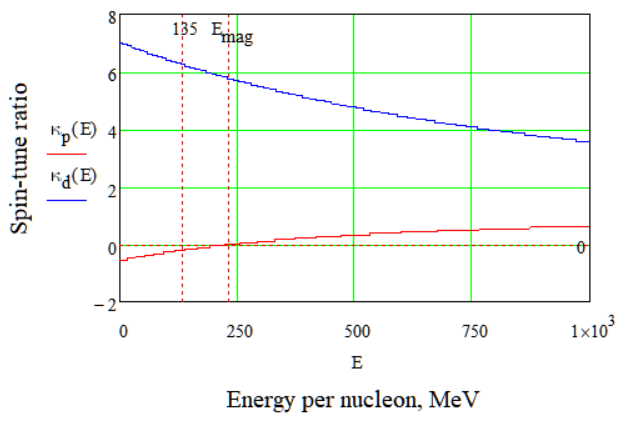
\includegraphics[width=0.58\textwidth]{YVSspin-tune_ratio}
  \caption{Spin-tune ratio
    $\kappa = \nu_{\mathrm{B}_{\perp}}/\nu_{\mathrm{E}}$ for deuteron and
    proton.}
  \label{fig:spin-tune}
\end{figure}

These fundamental differences lead to several important consequences for
lattice construction. Specifically, modifications are necessary to accommodate
both particle types. First, according to Eq.~\eqref{eq:deflection}, the direction of spin rotation
differs between protons and deuterons. This necessitates either switching the
polarity of the spin compensator's fields or rotating it by $\pi$ along the
longitudinal axis. Second, the minimal achievable spin compensator length, as
given by Eq.~\eqref{eq:length_min}, is longer for protons than for deuterons
at the optimal polarimeter energy. This discrepancy can be addressed by
lowering the experimental energy for protons (Fig.~\ref{fig:totallength}). At
a spin compensator length equivalent to that used for deuterons, the proton
energy should be reduced to \SI{73}{MeV}, and the analyzing power decreases by
a factor of 2--3. Third, two viable approaches for arranging additional EM fields are the
implementation of a Wien filter or an electrostatic deflector with a kicker.

\begin{figure}[htbp]
  \centering
  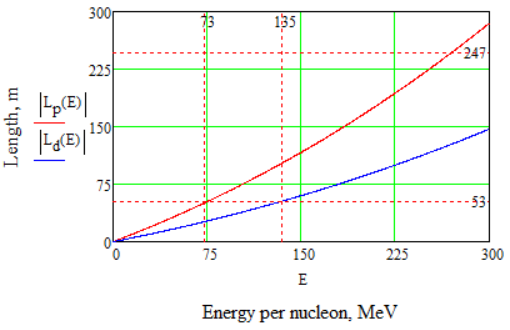
\includegraphics[width=0.58\textwidth]{YVStotal_length}
  \caption{Total length of the spin compensator versus energy per nucleon
    required to achieve a QFS lattice for deuteron and proton.}
  \label{fig:totallength}
\end{figure}

\subsubsection{Wien filter}

The Wien filter serves an important function in a particle accelerator,
designed to manipulate spin dynamics without altering the orbital trajectory of
particles by utilizing perpendicular electric and magnetic fields that cancel
each other out, resulting in zero net Lorentz force. As the EDM T-BMT term is
proportional to the Lorentz force, the Wien filter will not exert an EDM force
on the spin vector. It is EDM-transparent. It allows particles to move in a
straight line while enabling a precise correction of their spin orientations,
making it an ideal auxiliary device for experiments requiring spin
manipulation. It provides the conditions to facilitate spin navigation. The
filter's design ensures a net absence of deflection along the beamline,
minimizing additional space requirements in the ring's straight sections and
allowing for a classical sequential arrangement of ring elements.

It is usable for both deuterons and protons; for deuterons, it can be employed
directly at optimal energies, while for protons, the polarity must be switched
or the setup rotated by $\pi$ along the longitudinal axis and used at lower
energies (Figs.~\ref{fig:wf_vector_d}, \ref{fig:wf_vector_p},
\ref{fig:axion_diagram} and~\ref{fig:wien-filter}). This
flexibility allows for freedom in developing methods for studying spin dynamics
across different particle types. Overall, the Wien filter's ability to control
particle spin without perturbing orbital paths makes it an invaluable component
in advanced accelerator experiments.

\begin{figure}[htbp]
  \centering
  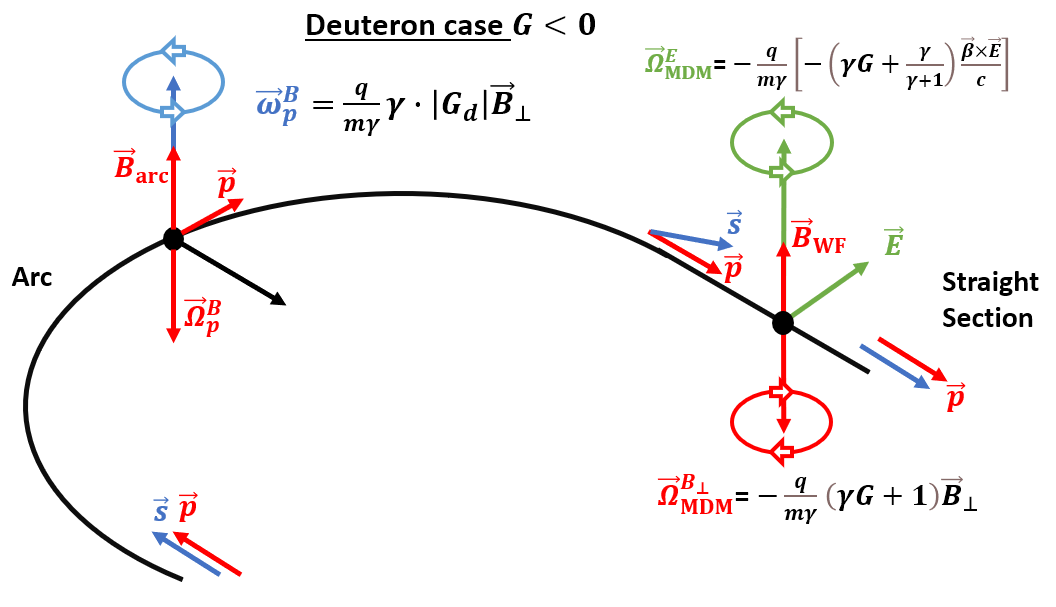
\includegraphics[width=0.92\textwidth]{YVSDeuteronWF_scheme}
  \caption{Vector scheme of the QFS turn with a Wien filter for the deuteron
    case $G<0$.}
  \label{fig:wf_vector_d}
\end{figure}

\begin{figure}[htbp]
  \centering
  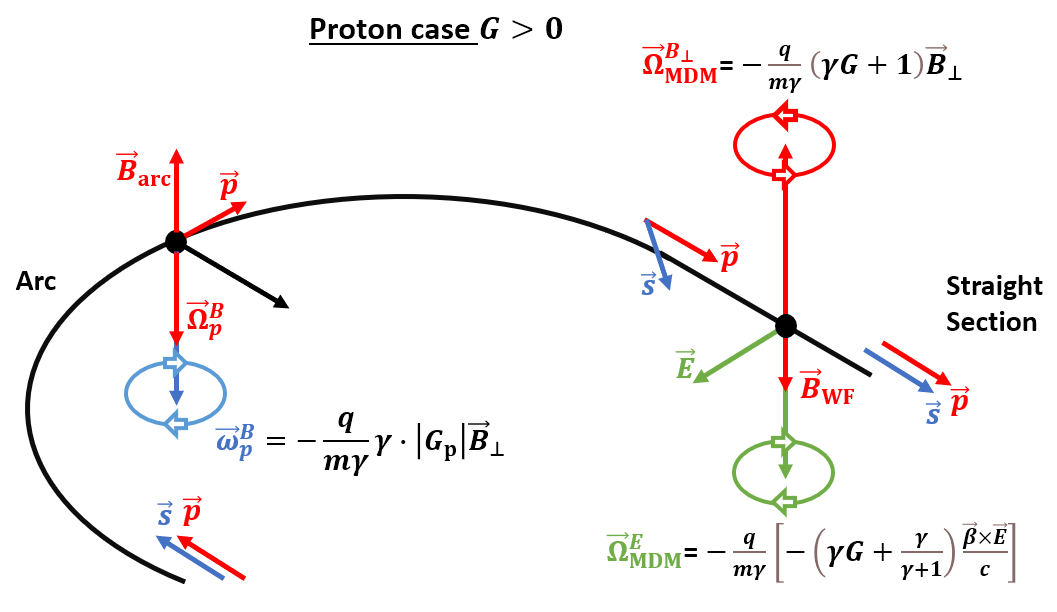
\includegraphics[width=0.92\textwidth]{YVSProtonWF_scheme}
  \caption{Vector scheme of the QFS turn with a Wien filter for the proton
    case $G>0$.}
  \label{fig:wf_vector_p}
\end{figure}

\begin{figure}[htbp]
  \centering
  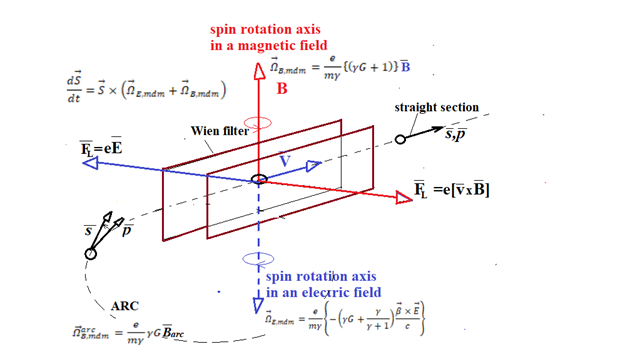
\includegraphics[width=0.88\textwidth]{YVSaxion_spin_diagram}
  \caption{Vector diagram of the spin transformation for the deuteron.}
  \label{fig:axion_diagram}
\end{figure}

\begin{figure}[htbp]
  \centering
  \begin{panel}{0.48\textwidth}
    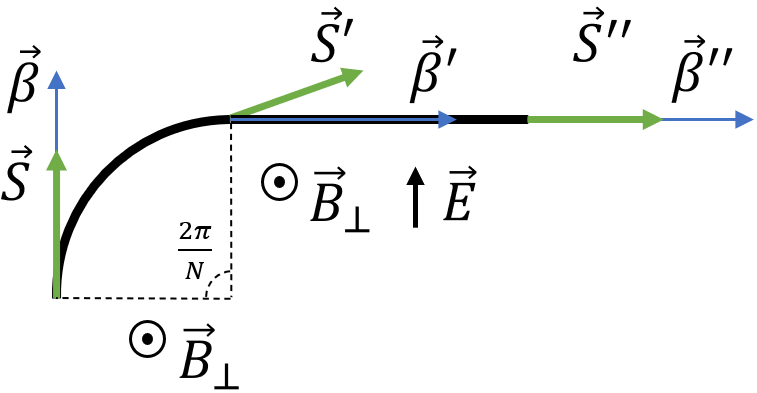
\includegraphics[width=\linewidth]{YVSwien-filter_deuteron}
  \end{panel}\hfill
  \begin{panel}{0.48\textwidth}
    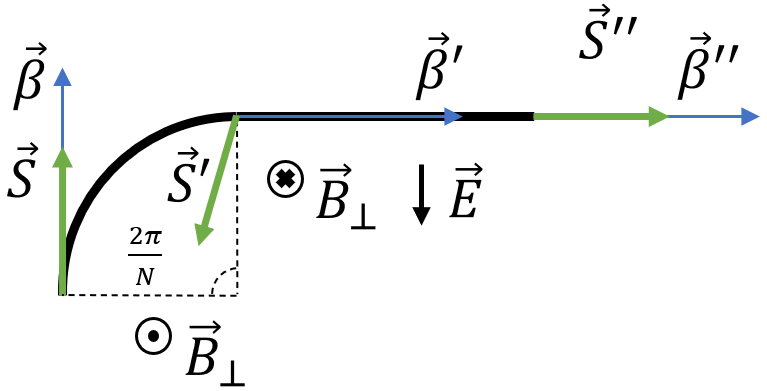
\includegraphics[width=\linewidth]{YVSwien-filter_proton}
  \end{panel}
  \caption{One-period conceptual scheme of a QFS lattice with Wien filters for
    deuterons (a) and protons (b).}
  \label{fig:wien-filter}
\end{figure}

\subsubsection{Electrostatic deflector with kicker}

The pure electrostatic deflector is designed to manipulate particle
trajectories and spin dynamics by creating a radial electric field with a
nonzero curvature. Unlike the Wien filter, this deflector requires an
additional kicker to compensate for orbital deviations, which increases the
overall length of the compensator. This setup is particularly useful for
creating bypass sections in addition to the native straight sections, allowing
for flexible experimental configurations (Fig.~\ref{fig:el-defdeuteron}). However, the distance between the spatial
assignment of equipment should be considered to enable the option with an
independent section. A key challenge is that each
type of particle requires a different curvature, which must be determined at
the outset of lattice design. Despite these complexities, the electrostatic
deflector with kicker offers a robust solution for controlling particle spin
and trajectory.

\begin{figure}[htbp]
  \centering
  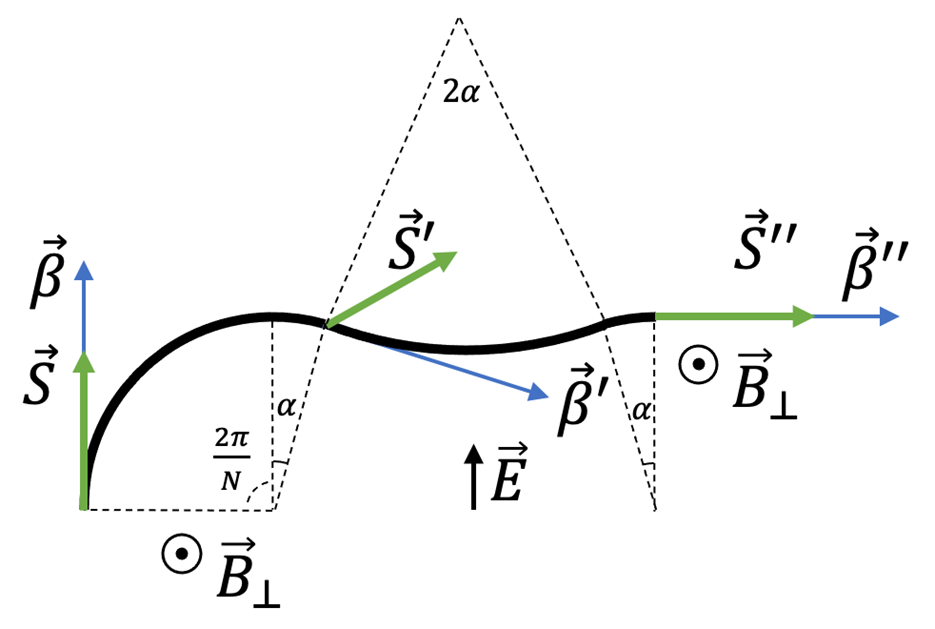
\includegraphics[width=0.7\textwidth]{YVSel-def_deuteron}
  \caption{One-period conceptual scheme of a QFS lattice with an electrostatic
    deflector and a kicker for deuterons.}
  \label{fig:el-defdeuteron}
\end{figure}

\subsection{Further research}

Currently, the proposed energy requirements for EDM studies are set at
\SI{270}{MeV} and lower, but specific conclusions regarding the arc spin
rotation have yet to be drawn. The primary condition is to achieve a momentum
rotation at a specific angle $\Phi_p^{\mathrm{arc}}$ with a corresponding
$\Phi_s^{\mathrm{arc}}$ for the spin. This can be accomplished by carefully selecting the magnetic field integral to ensure precise alignment of
momentum and spin dynamics. To maximize efficiency, the magnetic field should
be as strong as possible to minimize the effective arc length, in consideration
of the unique features of the lattice design. This approach not only optimizes
studies at the current energy range but also opens the possibility for other
polarized or non-polarized beam research at higher energies, potentially
reaching several GeV. The versatility of the QFS setup allows it to be
implemented in various lattice designs, including existing accelerator rings,
thereby facilitating advanced studies at elevated energy ranges.

Wien filters do not affect beam dynamics and influence only the spin motion.
This helps in converting the storage ring into a broadband axion
antenna~\cite{Nikolaev:2022wyi}.

The material of this section has been reported
in~\cite{Kolokolchikov:2026xbv,Senichev:2016rez,Senichev:2023vtx,Senichev:2024qtr,Senichev:2025jqf}.

% ===== 03-nica-bypass =====
\section{NICA collider with bypasses}
\label{sec:nica-bypass}

\subsection{Modified NICA lattice for the EDM search}

The NICA lattice was not designed for EDM research; hence the only option is
the quasi-frozen spin concept of Sec.~\ref{sec:qfs}, which can be realized for
deuterons. The adaptation strategy relies on two facts. First, the straight
sections of the collider are fully occupied by the equipment of the MPD and SPD
experiments. Second, these detectors and their interaction points are not
needed for the EDM search. The simplest solution is therefore to introduce
bypasses, as shown in Fig.~\ref{fig:bypass_layout}.

\begin{figure}[htbp]
  \centering
  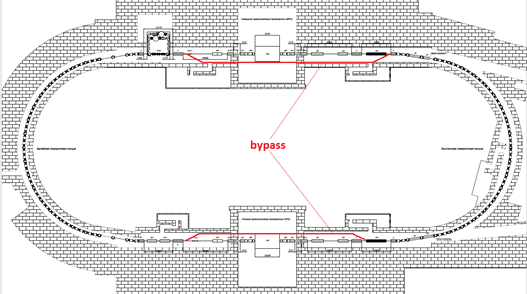
\includegraphics[width=0.75\textwidth]{YVSnica_bypass_layout}
  \caption{Modified NICA lattice for the EDM search with bypass insertions (red).}
  \label{fig:bypass_layout}
\end{figure}

The bypass sections avoid both detector interaction points and provide free
space for E+B elements. Owing to the zero Lorentz force, these elements are
transparent to the beam dynamics, while they rotate the spin opposite to its
rotation in the arcs and thus realize the quasi-frozen spin concept. Without
the interaction points, the two beams circulate in two uncoupled rings, which
doubles the data-taking rate.
Figures~\ref{fig:bypass_twiss} and~\ref{fig:bypass_da} show the Twiss functions
and the dynamic aperture in both transverse planes.

\begin{figure}[htbp]
  \centering
  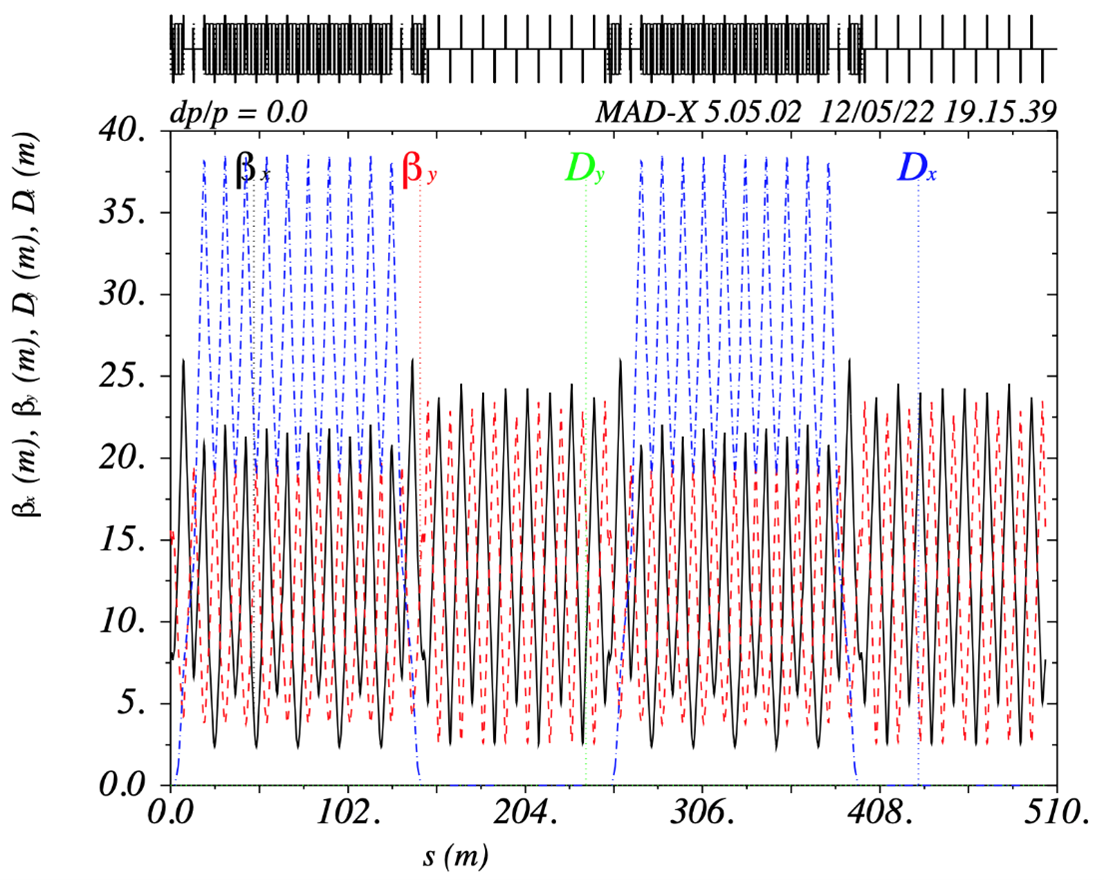
\includegraphics[width=0.7\textwidth]{YVSnica_bypass_twiss}
  \caption{Twiss functions of NICA with bypass insertions.}
  \label{fig:bypass_twiss}
\end{figure}

\begin{figure}[htbp]
  \centering
  \begin{panel}{0.48\textwidth}
    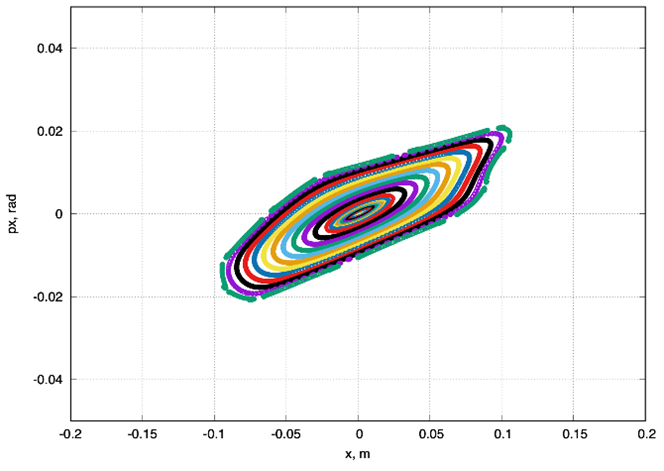
\includegraphics[width=\linewidth]{YVSnica_bypass_da_x}
  \end{panel}\hfill
  \begin{panel}{0.48\textwidth}
    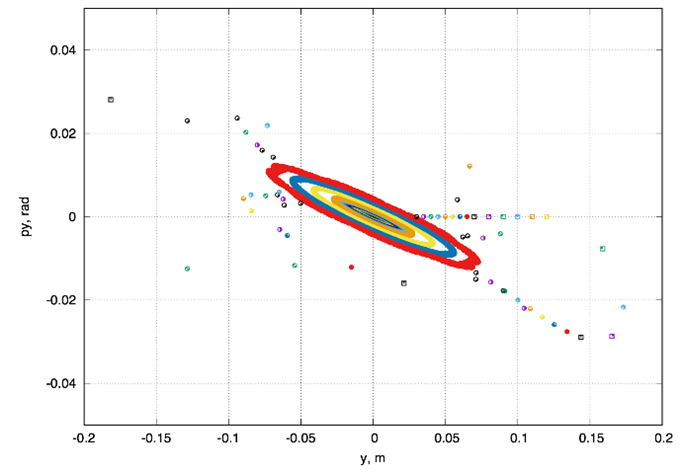
\includegraphics[width=\linewidth]{YVSnica_bypass_da_y}
  \end{panel}
  \caption{Dynamic aperture of NICA with bypass insertions in the horizontal (a)
    and vertical (b) planes.}
  \label{fig:bypass_da}
\end{figure}

The linear part of the dynamic aperture, about \SI{2000}{mm.mrad},
significantly exceeds the required value in both planes. For an electric field
limited to about \SI{100}{kV/cm}, Eq.~\eqref{eq:length_min} gives a total length of the
E+B elements of about 25--\SI{30}{m} per bypass, which is 30\% of the bypass
length. Spin-orbit tracking shows that the spin deviates from the momentum by
less than \ang{10}; the simulation for the three spin projections gives a
deviation within $\pm\ang{7.5}$. Despite this deviation, the polarization
asymmetry measured at the polarimeter location remains constant.

\subsection{Lattice parameters}

The polarimetry constraints~\cite{Kurilkin:2010ym} determine the choice of the
particle species and the experiment energy. The lattice is designed for
deuterons with a kinetic energy of \SI{240}{MeV}. The corresponding dipole
field and magnetic rigidity are listed in Table~\ref{tab:bypass_param}.

\begin{table}[htbp]
  \centering
  \caption{Main parameters of the experiment and the bypass lattice.}
  \label{tab:bypass_param}
  \begin{tabular}{ll}
    \toprule
    Particles & deuterons \\
    Dipole magnetic field & \SI{0.132}{T} \\
    Magnetic rigidity $B\rho$ & \SI{3.252}{T.m} \\
    Ring circumference & \SI{503.04}{m} \\
    Experiment energy & \SI{240}{MeV} \\
    \bottomrule
  \end{tabular}
\end{table}

\subsection{Bypass optics}

The arc geometry of the NICA ring is kept unchanged; only the fields in the
installed elements may be changed. NICA can therefore be used for different
experiments without a major rebuild of the lattice.

The NICA arc has a non-zero dispersion, and both the dispersion and its
derivative vanish at the arc ends. The straight sections are dispersion-free
along their whole length. The circumference of the original NICA ring is
$L_{acc} = \SI{503.04}{m}$ and the length of one arc is
$L_{arc} = \SI{142.15}{m}$, which leaves
$(L_{acc}-2L_{arc})/2 = \SI{109.6}{m}$ for each straight section. The bypass
channels contain an alternative straight section and sections with bending
dipoles. The dipoles deflect the beam by $\alpha = \ang{9}$; their field is
$B_{BP} = \SI{1}{T}$ and their length is $L^{BP}_{dip} = \SI{50}{cm}$. The
alternative straight section is displaced by \SI{1}{m} from the original one,
so the length of the bypass channel is
$L_{BP} = \SI{1}{m}/\sin\alpha \approx \SI{6.4}{m}$. The general layout of
the bypass channels is shown in Fig.~\ref{fig:bypass_layout}.

The bending magnets perturb the dispersion function. At least two focusing
quadrupoles in the bypass channel are therefore needed to suppress the
dispersion at its exit and to keep the whole straight section
dispersion-free. One or three defocusing quadrupoles can be used to keep the
beta functions periodic and symmetric. Two cases with adapted straight
sections, identical to the arcs but without dipoles, are considered first;
this simplifies the modeling of an ideal regular lattice. Finally, a
realistic lattice with a fully regular FODO straight section is considered.

\paragraph{Bypass with three quadrupoles.}
In this case the bypass channel contains the minimum of three quadrupoles: two
focusing quadrupoles QBP1 and one defocusing quadrupole QBP2
(Fig.~\ref{fig:bypass_scheme_3q}). The arc is matched to the bypass channel by
three quadrupoles QM1, QM2 and QM3 (matching section M1), and the bypass is
matched to the straight section by the same quadrupoles (M2). This is possible
because of the symmetry between the arc and the straight section built into
the original lattice. The section lengths are given in
Fig.~\ref{fig:bypass_scheme_3q} and Table~\ref{tab:bypass_lengths}. The ring
circumference becomes $L^{acc}_{3quad} = \SI{503.46}{m}$.

\begin{figure}[htbp]
  \centering
  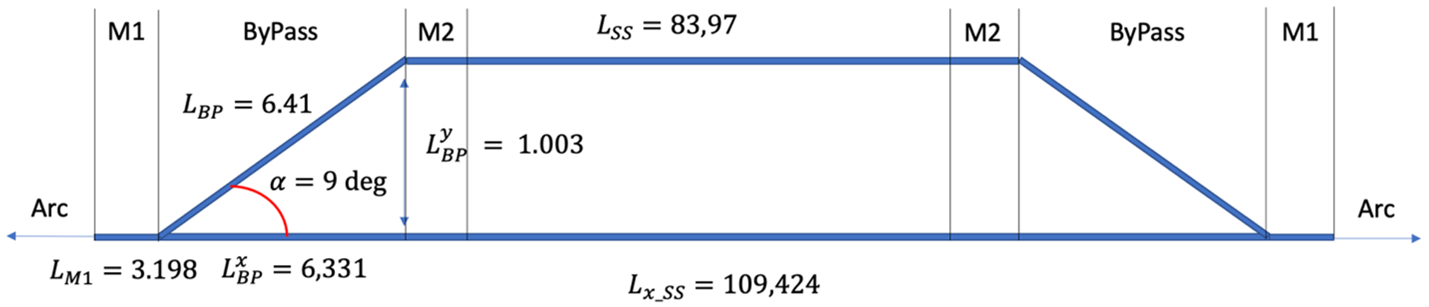
\includegraphics[width=\textwidth]{YVSbypass_scheme_3q}
  \caption{Layout of the bypass with three quadrupoles.}
  \label{fig:bypass_scheme_3q}
\end{figure}

Figure~\ref{fig:bypass_twiss_3q} shows the Twiss functions; the black lines
mark the channel boundaries. The maximum of $\beta_y$ is located at the center
of the channel and can be large compared with $\beta_x$. For this reason, a
bypass with five quadrupoles is also considered.

\begin{figure}[htbp]
  \centering
  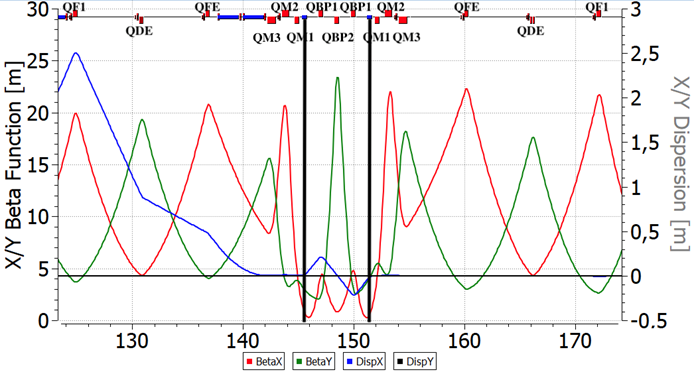
\includegraphics[width=0.7\textwidth]{YVSbypass_twiss_3q}
  \caption{Twiss functions of the bypass with three quadrupoles. The black lines
    show the positions of the bypass bending magnets.}
  \label{fig:bypass_twiss_3q}
\end{figure}

\paragraph{Bypass with five quadrupoles.}
Here the bypass channel contains five quadrupoles of two families, focusing
QBP1 and defocusing QBP2. The channel becomes longer,
$L^{BP}_{5quad} = \SI{9.35}{m}$, and the displacement increases to
\SI{1.46}{m} (Fig.~\ref{fig:bypass_scheme_5q}). The matching sections M1 and M2
are still identical but consist of two quadrupoles, QM1 and QM2, which keep the
Twiss functions regular. The circumference increases to
$L^{acc}_{5quad} = \SI{510.02}{m}$. As Fig.~\ref{fig:bypass_twiss_5q} shows,
the maximum of $\beta_y$ at the channel center becomes smaller, whereas the
maximum of the dispersion grows from $D_x^{3quad}\sim\SI{0.2}{m}$ to
$D_x^{5quad}\sim\SI{0.5}{m}$. This case therefore has to be adapted to the
real lattice.

\begin{figure}[htbp]
  \centering
  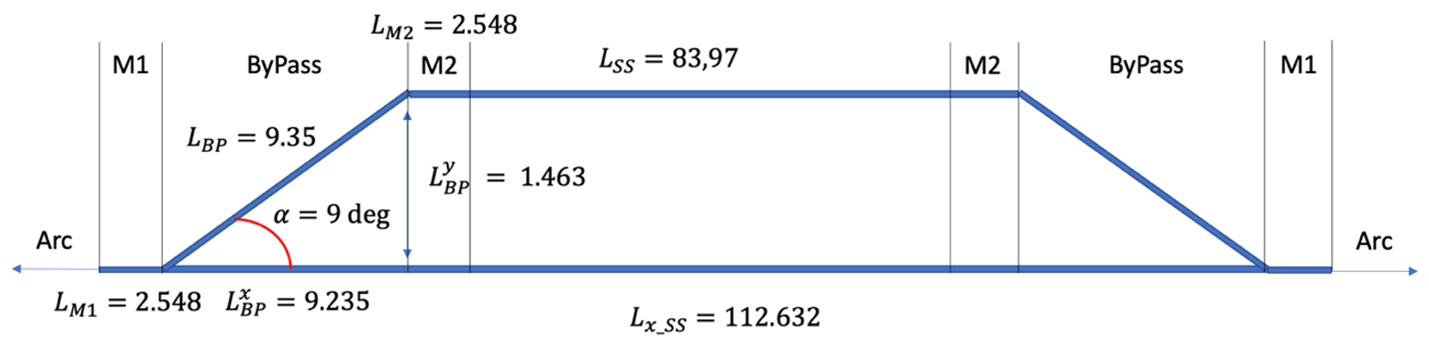
\includegraphics[width=\textwidth]{YVSbypass_scheme_5q}
  \caption{Layout of the bypass with five quadrupoles.}
  \label{fig:bypass_scheme_5q}
\end{figure}

\begin{figure}[htbp]
  \centering
  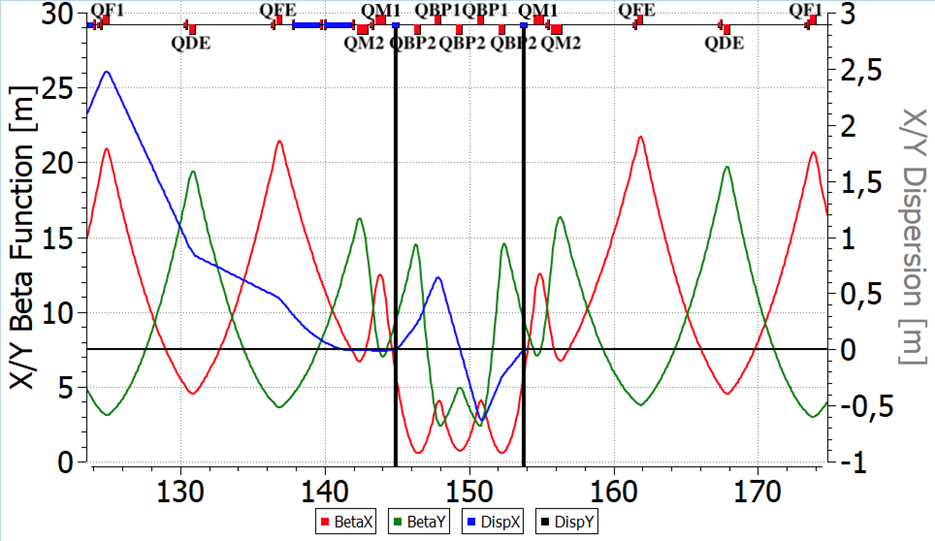
\includegraphics[width=0.7\textwidth]{YVSbypass_twiss_5q}
  \caption{Twiss functions of the bypass with five quadrupoles. The black lines
    show the positions of the bypass bending magnets.}
  \label{fig:bypass_twiss_5q}
\end{figure}

\paragraph{Realistic lattice.}
Based on these two cases, a lattice as close as possible to the real machine
has been designed. It has a fully regular straight section, which becomes
shorter, $L^{BP}_{SS} = \SI{80.71}{m}$ (Fig.~\ref{fig:bypass_scheme_real}). The
bypass channel contains five quadrupoles and displaces the alternative
straight section by \SI{1.46}{m} from the original one. Different matching
sections M1 and M2 are used to compensate the asymmetry between the arc and
the straight section. The Twiss functions of one half of the NICA ring with
bypasses are shown in Fig.~\ref{fig:bypass_twiss_half}; the Wien filters are
placed at the center of the straight section. All Twiss functions were
computed with OptiM~\cite{Lebedev:OptiM}. The lengths and tunes of all
versions are summarized in Table~\ref{tab:bypass_lengths}.

\begin{figure}[htbp]
  \centering
  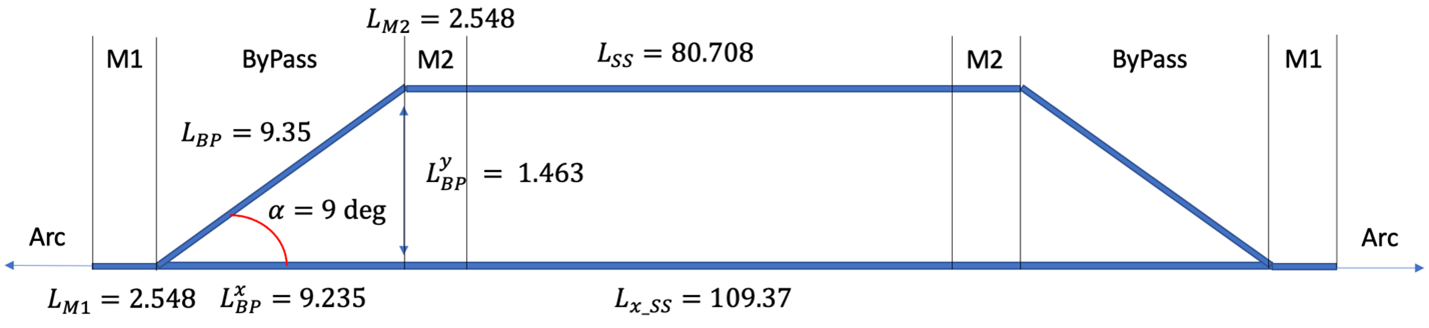
\includegraphics[width=\textwidth]{YVSbypass_scheme_real}
  \caption{Layout of the bypass in the realistic lattice.}
  \label{fig:bypass_scheme_real}
\end{figure}

\begin{figure}[htbp]
  \centering
  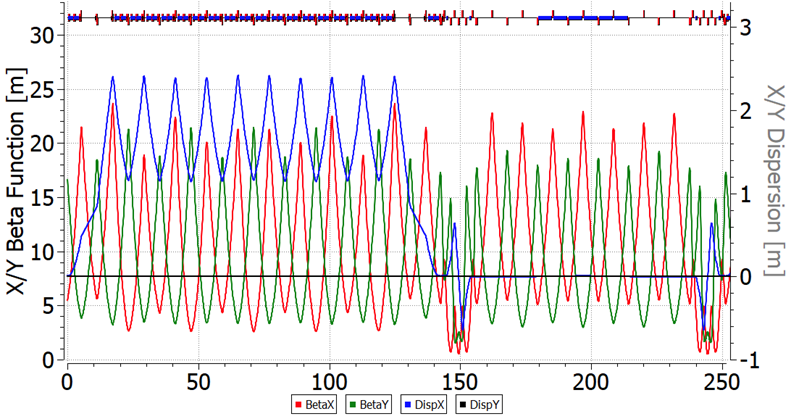
\includegraphics[width=0.75\textwidth]{YVSbypass_twiss_half}
  \caption{Twiss functions of one half of the NICA ring with bypasses. The Wien
    filters are located in the straight section.}
  \label{fig:bypass_twiss_half}
\end{figure}

\begin{table}[htbp]
  \centering
  \caption{Ring circumference, lengths of the individual sections and betatron
    tunes $Q_x/Q_y$ of the lattice versions.}
  \label{tab:bypass_lengths}
  \small
  \setlength{\tabcolsep}{4pt}
  \begin{tabular}{lccccc}
    \toprule
    Lattice & \makecell{Circumfe-\\rence, m} & \makecell{Straight\\section, m}
      & \makecell{Bypass,\\m} & \makecell{Matching\\section, m} & $Q_x/Q_y$ \\
    \midrule
    NICA (ion mode) & 503.04 & 109.6 & -- & -- & 9.44/9.44 \\
    3 quadrupoles & 503.46 & 83.97 & 6.41 & 3.198 & 13.8/11.8 \\
    5 quadrupoles & 510.0 & 83.97 & 9.35 & 2.548 & 13.44/11.44 \\
    Realistic & 503.5 & 80.70 & 9.35 & 2.548 & 12.8/11.8 \\
    \bottomrule
  \end{tabular}
\end{table}

\subsection{Natural chromaticity and dynamic aperture}

This subsection addresses the stability of the orbital motion, namely, the
correction of the natural chromaticity of the NICA bypass lattice. The
chromaticity is the dependence of the betatron tune $Q$ on the momentum
deviation $\delta$~\cite{Guiducci:1992kb}:
\begin{equation}
  Q' = \frac{dQ}{d\delta} .
\end{equation}
The natural chromaticity is produced by the quadrupoles at locations with
non-zero beta function:
\begin{equation}
  \frac{\partial Q_x}{\partial\delta} = -\frac{1}{4\pi}\int_0^L \beta_x(s)\,k_x(s)\,ds,
\end{equation}
where $\beta_x(s)$ is the beta function at the quadrupole and $k_x(s)$ is the
quadrupole gradient. The natural chromaticity can be corrected with
sextupoles:
\begin{equation}
  \frac{\partial Q_x}{\partial\delta} = \frac{1}{4\pi}\int_0^L \beta_x(s)\,r(s)\,D(s)\,ds,
\end{equation}
where $D(s)$ is the dispersion function and $r(s)$ is the sextupole gradient.
Correction is possible only if the sextupoles are placed where both the
dispersion and the beta function are non-zero.

Since the arc lattice is regular, the beta and dispersion functions are
regular along the arc as well, except at the arc ends. There the dispersion is
suppressed with the missing-magnet method, which breaks the regularity of the
Twiss functions (Fig.~\ref{fig:bypass_twiss_half}). Two essentially different
sextupole families can thus be placed in the regular part of the arc:
(1)~at the maximum of $D$ and $\beta_x$ and the minimum of $\beta_y$, and
(2)~at the minimum of $D$ and $\beta_x$ and the maximum of $\beta_y$.

Figure~\ref{fig:bypass_tune_dp} shows the betatron tune versus the energy
deviation for the natural chromaticity and for the chromaticity corrected with
two sextupole families. Figure~\ref{fig:bypass_da_sext} shows the dynamic
aperture without sextupoles and with the chromaticity corrected. The tracking
was performed with COSY Infinity~\cite{Makino:2006sx}. The main parameters are
listed in Table~\ref{tab:bypass_chrom}.

\begin{table}[htbp]
  \centering
  \caption{Chromaticity of the NICA ring with bypasses.}
  \label{tab:bypass_chrom}
  \begin{tabular}{lc}
    \toprule
    Natural chromaticity $\xi_x/\xi_y$ & $-17/{-17}$ \\
    Corrected chromaticity $\xi_x/\xi_y$ & $-7\times10^{-6}/7\times10^{-6}$ \\
    Number of sextupole families & 2 \\
    \bottomrule
  \end{tabular}
\end{table}

\begin{figure}[htbp]
  \centering
  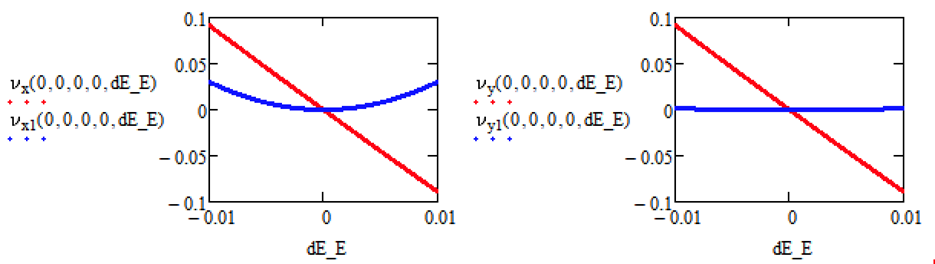
\includegraphics[width=0.85\textwidth]{YVSbypass_tune_vs_dp}
  \caption{Betatron tune shift versus the energy deviation in the horizontal
    (left) and vertical (right) planes. Red: natural chromaticity; blue:
    corrected chromaticity.}
  \label{fig:bypass_tune_dp}
\end{figure}

\begin{figure}[htbp]
  \centering
  \begin{panel}{0.48\textwidth}
    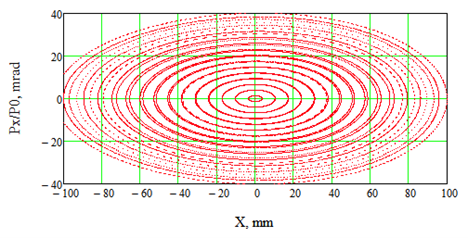
\includegraphics[width=\linewidth]{YVSbypass_da_nat_x}
  \end{panel}\hfill
  \begin{panel}{0.48\textwidth}
    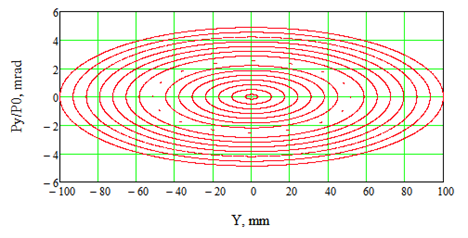
\includegraphics[width=\linewidth]{YVSbypass_da_nat_y}
  \end{panel}\\[4pt]
  \begin{panel}{0.48\textwidth}
    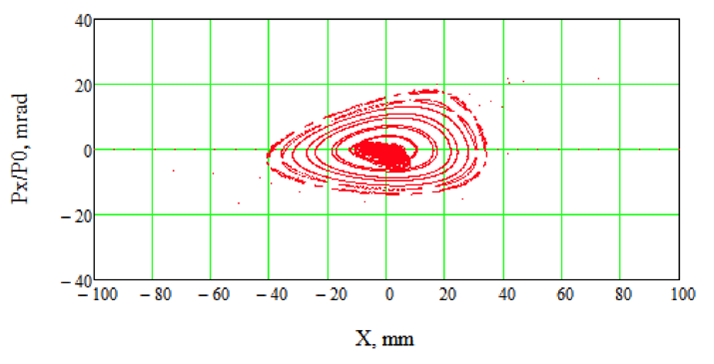
\includegraphics[width=\linewidth]{YVSbypass_da_corr_x}
  \end{panel}\hfill
  \begin{panel}{0.48\textwidth}
    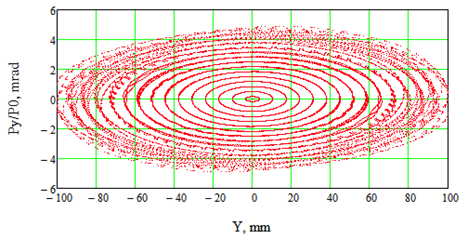
\includegraphics[width=\linewidth]{YVSbypass_da_corr_y}
  \end{panel}
  \caption{Dynamic aperture of the NICA ring with bypasses: (a), (b) natural
    chromaticity without sextupoles; (c), (d) chromaticity corrected with two
    sextupole families. Left: horizontal plane; right: vertical plane.}
  \label{fig:bypass_da_sext}
\end{figure}

\subsection{Spin-orbit motion with optimized Wien filters}

The modification of the lattice is intended primarily for EDM research. This
implies that the ring must operate in the quasi-frozen spin mode and that the
spin coherence time of the beam must be long enough. The first requirement is
met by placing Wien filters in the straight sections; the standard way to meet
the second one is to use several sextupole families that correct the betatron
and spin chromaticities. Both points were studied numerically with COSY
Infinity~\cite{Makino:2006sx}.

In the standard formalism, the spin transfer matrix is an SO(3) rotation
$T(\nu, \bar{n})$ parametrized by the normalized spin precession frequency
(spin tune) $\nu$ and the invariant spin axis $\bar{n}$. If the quasi-frozen
spin condition holds, $T$ is the identity matrix and $\nu = 0$. In the
proposed lattice this is achieved by tuning the electric field of the E+B
elements, while the magnetic field is chosen so as to keep the closed orbit
unchanged. The simulation shows that the spin tune of the reference particle
$\nu_0$ can indeed be set to zero (Fig.~\ref{fig:bypass_spintune}). The spin
deviates by a small angle in the arc and recovers its orientation in the Wien
filters of the straight section (Fig.~\ref{fig:bypass_spin_components}).

\begin{figure}[htbp]
  \centering
  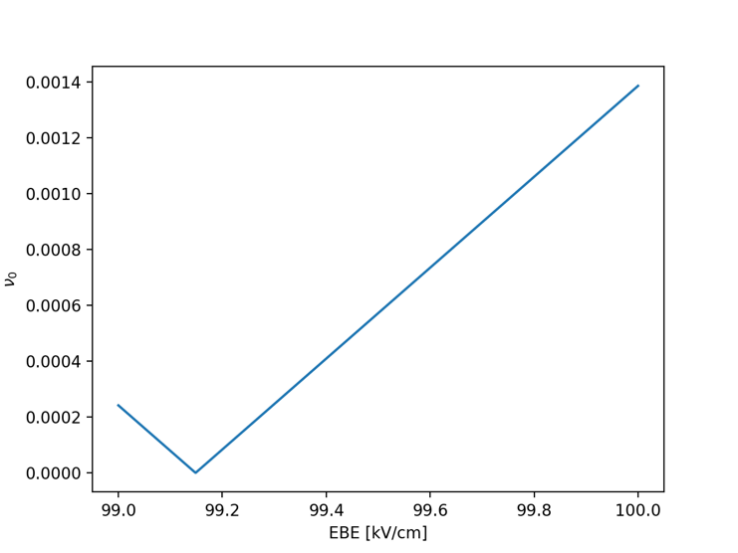
\includegraphics[width=0.6\textwidth]{YVSbypass_spintune_ebe}
  \caption{Spin tune $\nu_0$ of the reference particle versus the electric field
    of the E+B elements.}
  \label{fig:bypass_spintune}
\end{figure}

\begin{figure}[htbp]
  \centering
  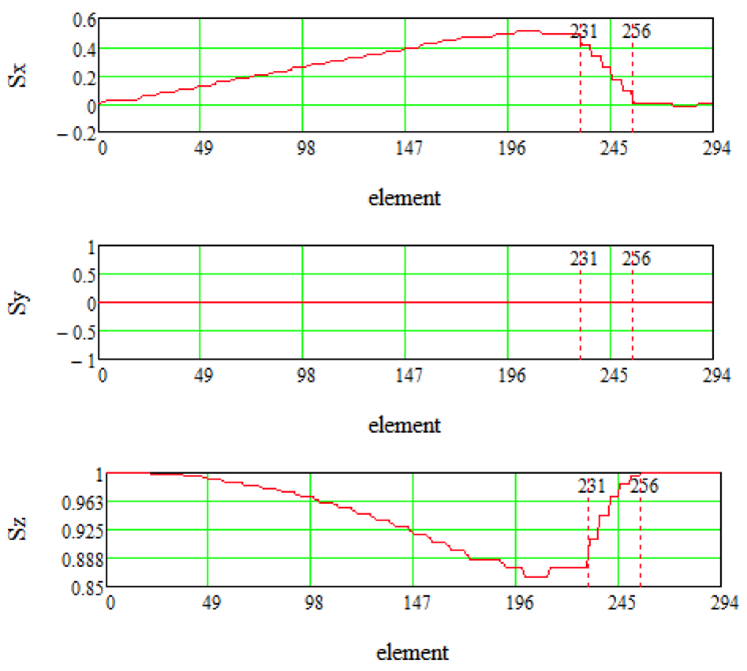
\includegraphics[width=0.7\textwidth]{YVSbypass_spin_components}
  \caption{Spin components $S_x$, $S_y$, $S_z$ of the reference particle along
    one half of the ring (arc and straight section).}
  \label{fig:bypass_spin_components}
\end{figure}

The spin chromaticity is the dependence of the spin precession frequency on the
particle orbit length~\cite{Senichev:2021wcy}. Because of it, the spins of the
beam particles spread around the invariant spin axis $\bar{n}$. This process,
called spin decoherence~\cite{Melnikov:2023cms,Aksentev:2022boh,Aksentev:2022wyn},
is irrelevant for experiments with a non-zero expected polarization along
$\bar{n}$. In EDM experiments, however, the polarization component orthogonal
to $\bar{n}$ is of interest; its expectation value is zero, hence the
importance of the spin coherence time (SCT).

The spin chromaticity of the beam can be compensated with sextupole families
to a level that provides a sufficiently long spin coherence time
(Fig.~\ref{fig:bypass_spin_sext}). Classically, three sextupole families placed
at the maxima of $\beta_x$, $\beta_y$ and $D$ should be used, but the lattice
under study does not allow an efficient separation of all three Twiss
functions. It was also found that the betatron and spin chromaticities cannot
be compensated simultaneously in this combined lattice; this problem is
discussed in the next subsection.

\begin{figure}[htbp]
  \centering
  \begin{panel}{0.49\textwidth}
    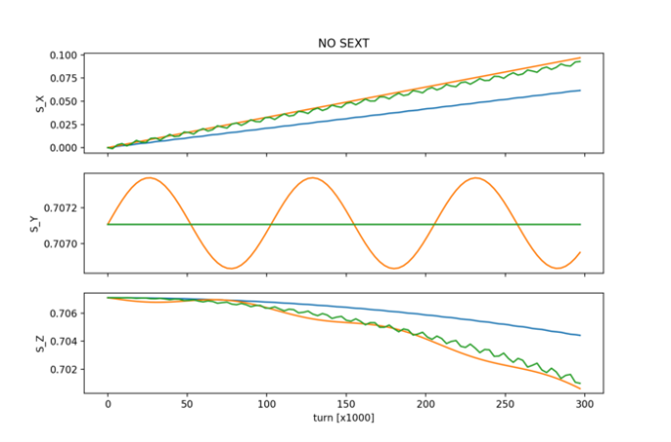
\includegraphics[width=\linewidth]{YVSbypass_spin_nosext}
  \end{panel}\hfill
  \begin{panel}{0.49\textwidth}
    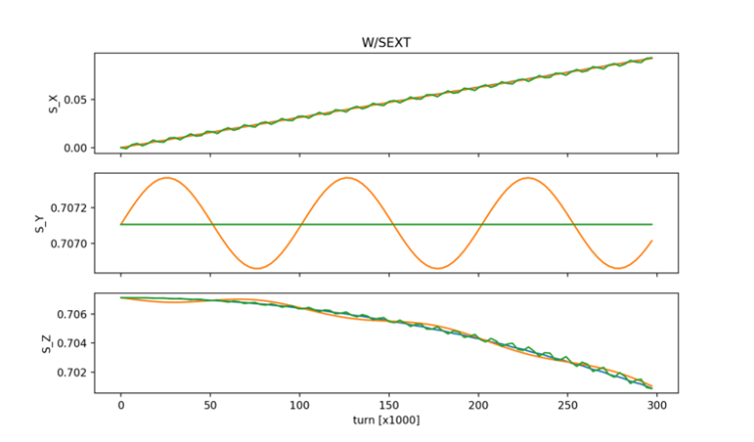
\includegraphics[width=\linewidth]{YVSbypass_spin_sext}
  \end{panel}
  \caption{Spin components versus the number of turns for particles with
    different initial offsets, without (a) and with (b) sextupole families.}
  \label{fig:bypass_spin_sext}
\end{figure}

\subsection{Betatron chromaticity and spin coherence}

According to the theory of Ref.~\cite{Melnikov:2023_jetpl_decoherence}, the main cause of
spin decoherence is the deviation of the particle energy from the equilibrium
value:
\begin{equation}
  \Delta\delta_{eq} = \frac{\gamma_s^2}{\gamma_s^2\alpha_0-1}
  \left[\frac{\delta_m^2}{2}\left(\alpha_1+\frac{3}{2}\frac{\beta_s^2}{\gamma_s^2}
  -\frac{\alpha_0}{\gamma_s^2}+\frac{1}{\gamma_s^4}\right)
  + \left(\frac{\Delta L}{L}\right)_\beta\right],
  \label{eq:delta_eq}
\end{equation}
\begin{equation}
  \left(\frac{\Delta L}{L}\right)_\beta = \frac{\pi}{2L}\left[\epsilon_x\nu_x+\epsilon_y\nu_y\right].
  \label{eq:dl_beta}
\end{equation}
The energy level around which the particle oscillates is called the effective
energy. To eliminate the effect of the momentum spread on the orbit
lengthening completely, the factor
$\kappa = \eta_1 = \alpha_1+\frac{3}{2}\frac{\beta_s^2}{\gamma_s^2}
-\frac{\alpha_0}{\gamma_s^2}+\frac{1}{\gamma_s^4}$
in Eq.~\eqref{eq:delta_eq} must vanish. In addition, the orbit lengthening
due to the betatron motion must be compensated as well. Both are achieved with
three independent sextupole families placed at the maxima of the beta and
dispersion functions. With sextupoles in the lattice, Eq.~\eqref{eq:dl_beta}
takes the more general form~\cite{Melnikov:2022xao}
\begin{equation}
  \left(\frac{\Delta L}{L}\right)_\beta = -\frac{\pi}{L}\left[\epsilon_x\xi_x+\epsilon_y\xi_y\right].
  \label{eq:dl_beta_sext}
\end{equation}

\paragraph{Magnetic ring.}
To study this effect, a purely magnetic ring without electric elements is
considered first; similar calculations were carried out for the COSY ring in
J\"ulich~\cite{Melnikov:2022xao}. This ring is a version of NICA in which the
arcs are unchanged and the straight sections are regular FODO cells matched to
the arcs with two quadrupoles. The sensitivity of the lattice to the sextupole
strengths $r_f$ and $r_d$ is considered. The sextupole layout is shown in
Fig.~\ref{fig:arc_sext}; here the families SF1 and SF2 are identical and form
one focusing family.

\begin{figure}[htbp]
  \centering
  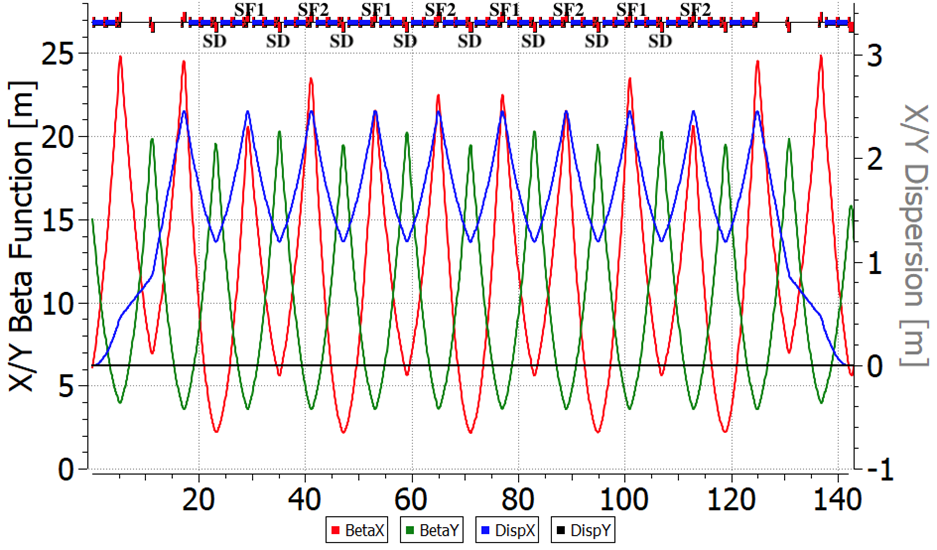
\includegraphics[width=0.75\textwidth]{YVSnica_arc_sextupoles}
  \caption{NICA collider arc with the sextupole layout.}
  \label{fig:arc_sext}
\end{figure}

\begin{equation}
  \left\{
  \begin{aligned}
    \xi_x &= -13.302 + 4522.234\, r_f + 527.934\, r_d,\\
    \xi_y &= -13.337 - 944.735\, r_f - 2214.642\, r_d,\\
    \alpha_1 &= 0.037 - 16.617\, r_f - 2.537\, r_d .
  \end{aligned}
  \right.
  \label{eq:sext_response}
\end{equation}
Two sextupole families cannot optimize all three parameters of the spin-orbit
motion. Either the pair $(\xi_x, \xi_y)$ or the pair $(\xi_y, \alpha_1)$ can be
tuned. The second choice is probably less practical, because $\alpha_1$
changes only weakly and the energy contribution to the spin tune spread can be
reduced by beam cooling.

In a purely magnetic lattice, the motion in the $x$--$\delta$ plane is fully
described by the theory. In the vertical plane, spin resonances may contribute
to the spread of the spin precession frequencies.

As Figs.~\ref{fig:mag_dnu}(a)--(c) show, the optimum of the spin chromaticity
does not coincide with that of the betatron chromaticity. Without
optimization, $\Delta\nu_s\sim10^{-8}$ at $f_{rev}\sim\SI{1}{MHz}$ gives an SCT
of about \SI{100}{s}, which is insufficient for the EDM experiment. The
vertical chromaticity must therefore be optimized while the dynamic aperture is
preserved. A change of $\kappa$ by about $\pm1$ is not decisive for the SCT.

\begin{figure}[htbp]
  \centering
  \begin{panel}{0.32\textwidth}
    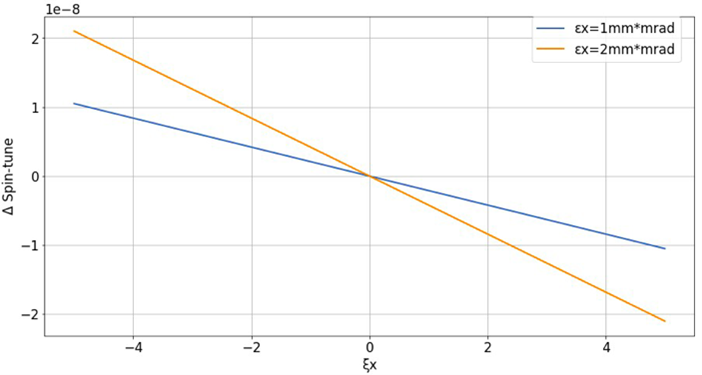
\includegraphics[width=\linewidth]{YVSmag_dnu_xix}
  \end{panel}\hfill
  \begin{panel}{0.32\textwidth}
    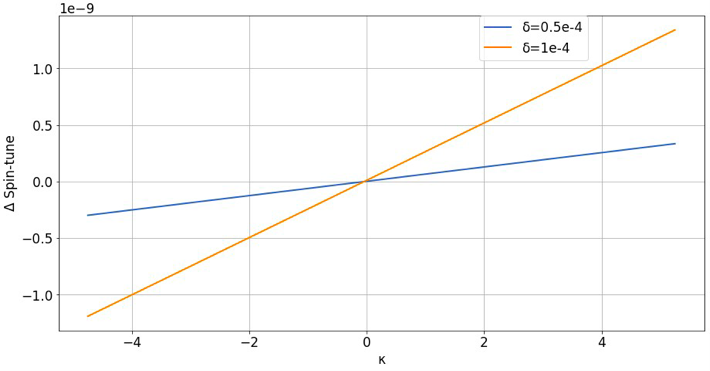
\includegraphics[width=\linewidth]{YVSmag_dnu_kappa}
  \end{panel}\hfill
  \begin{panel}{0.32\textwidth}
    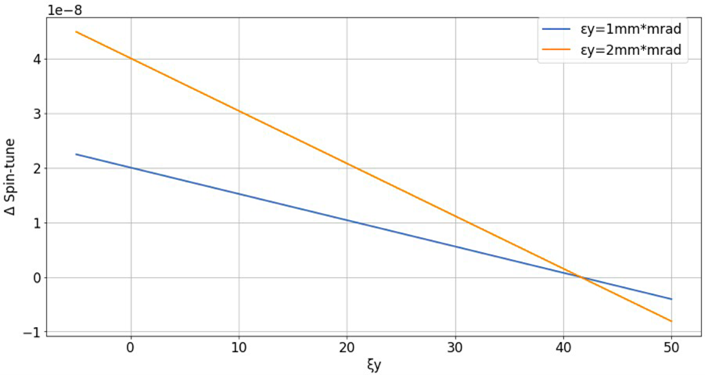
\includegraphics[width=\linewidth]{YVSmag_dnu_xiy}
  \end{panel}
  \caption{Purely magnetic ring: spin tune spread (a) versus the horizontal
    chromaticity for particles injected with different radial offsets;
    (b) versus $\kappa=\eta_1$ for particles with an energy offset;
    (c) versus the vertical chromaticity for particles with a vertical
    offset.}
  \label{fig:mag_dnu}
\end{figure}

As noted above, spin resonances produce an additional spread of the spin
precession frequencies $\Delta\nu_s$ in the vertical plane. At the working
point $\gamma G = 0.16$, the nearest resonance is the intrinsic betatron
resonance $\gamma G = 10 - Q_y = 0.2$. For a resonance strength
$\varepsilon = 10^{-4}$ and a detuning $\delta = 0.04$, the expected spread
due to the resonance is
\begin{equation}
  \Delta\nu_s = \delta - \sqrt{\delta^2+\varepsilon^2} \sim 1.2\times10^{-7}.
\end{equation}
This value estimates $\Delta\nu_s$ at $\xi_y = 0$ in
Fig.~\ref{fig:mag_dnu}(c). Increasing the vertical chromaticity reduces the
spread of the spin precession frequencies through the betatron orbit
lengthening. A simple estimate for a particle with
$\varepsilon_y\sim\SI{1}{mm.mrad}$ and $\xi_y = 40$ gives
\begin{equation}
  \Delta\nu_s = \nu_s\left(\frac{\Delta L}{L}\right)_\beta
  = -\frac{\gamma G\pi}{L}\,\varepsilon_y\xi_y = -4\times10^{-8},
\end{equation}
which is what is needed to suppress the typical spin tune spread at
$\xi_y = 0$ in Fig.~\ref{fig:mag_dnu}(c).

\paragraph{Lattice with Wien filters.}
As Figs.~\ref{fig:wf_dnu}(a)--(c) show, in a ring with electrostatic fields the
optima of the betatron and spin chromaticities do not coincide either in the
$x$--$\delta$ plane or in the vertical plane. As in the magnetic ring, the
preferred option for minimizing spin decoherence is to compensate the pair
$(\xi_x, \xi_y)$ for the beam parameters given above. The residual spread
$\Delta\nu_s\sim10^{-9}$ in the energy plane gives an SCT of about
\SI{1000}{s}, which is sufficient for the EDM experiment. Moreover,
measurements of $(\xi_x, \xi_y)$ are routine in storage rings, unlike
measurements of $\alpha_1$; with two sextupole families it is therefore
reasonable to optimize the pair $(\xi_x, \xi_y)$.

\begin{figure}[htbp]
  \centering
  \begin{panel}{0.32\textwidth}
    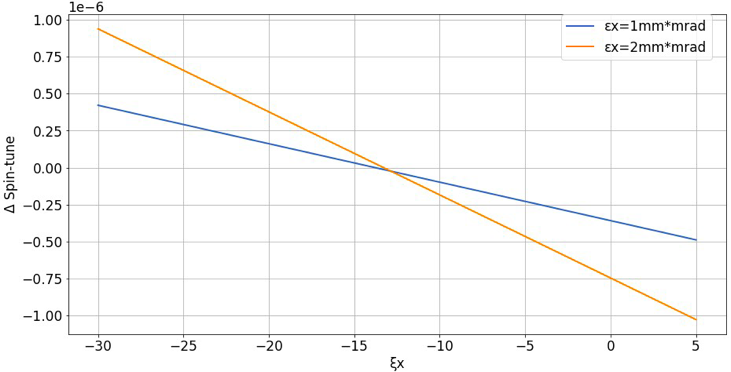
\includegraphics[width=\linewidth]{YVSwf_dnu_xix}
  \end{panel}\hfill
  \begin{panel}{0.32\textwidth}
    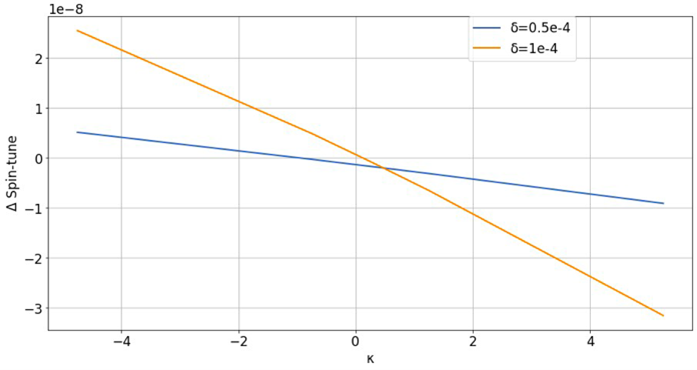
\includegraphics[width=\linewidth]{YVSwf_dnu_kappa}
  \end{panel}\hfill
  \begin{panel}{0.32\textwidth}
    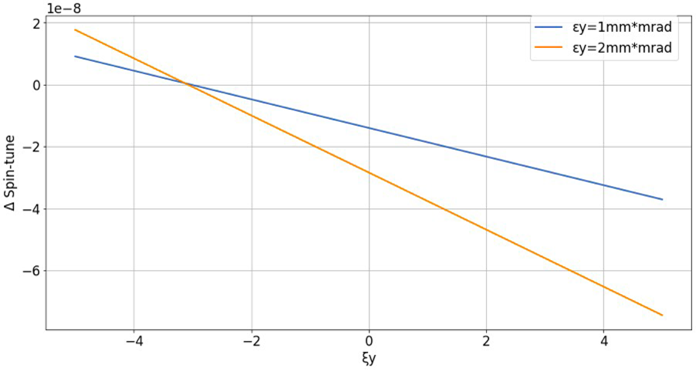
\includegraphics[width=\linewidth]{YVSwf_dnu_xiy}
  \end{panel}
  \caption{Ring with Wien filters: spin tune spread (a) versus the horizontal
    chromaticity for particles injected with different radial offsets;
    (b) versus $\kappa=\eta_1$ for particles with an energy offset;
    (c) versus the vertical chromaticity for particles with a vertical
    offset.}
  \label{fig:wf_dnu}
\end{figure}

The mismatch between the optima of the betatron and spin chromaticities in the
$x$--$\delta$ plane of a ring with electrostatic fields is explained by the
particle motion in the electric field. A radial displacement of a particle in
a deflector with a radial field changes the particle energy. This follows from
the potential nature of the field and couples the orbital motion to the
particle energy.

\paragraph{NICA with bypasses.}
For the modified NICA ring with bypasses and Wien filters described above, the
betatron chromaticity and the spin coherence were optimized separately.

To correct the betatron chromaticity, two sextupole families are needed, as
shown above: one near the focusing quadrupoles and the other near the
defocusing quadrupoles. The natural chromaticity of the NICA ring with
bypasses is $\xi_{x,y} = -17/{-17}$. After the correction, the spin precession
frequency can be followed in Fig.~\ref{fig:bypass_nu}: the red line shows the
natural chromaticity and the blue dotted line shows the chromaticity corrected
to zero. For this case, spin tracking over $3\times10^5$ turns was performed
for particles with different initial offsets in $x$, $y$ and $\delta$ and with
the initial spin $\vec{S}_0$ at \ang{45} in the $y$--$z$ plane
(Fig.~\ref{fig:bypass_spin_sext}).

The key quantity is the spin precession frequency, which in general depends on
the coordinates and the energy. The dominant contribution is the quadratic
term in the expansion of the spin precession frequency, as seen in
Fig.~\ref{fig:bypass_nu} for both the natural and the corrected
chromaticity.

To obtain spin coherence, the quadratic terms of the expansion were
compensated with two focusing sextupole families. These families, however,
are linearly dependent, because they are located at positions with equal
values of the beta and dispersion functions (Fig.~\ref{fig:arc_sext}), which
is typical of lattices with regular arcs. COSY Infinity cannot operate near a
zero spin precession frequency: the spin transfer matrix becomes degenerate
near the resonance and the code fails. The lattice was therefore detuned from
the resonance to $\nu_s\sim10^{-4}$, while the particles were still required to
precess synchronously, i.e., coherently. In this approach the chromaticity is
not controlled; its value is only monitored, and with the spin chromaticity
corrected it equals $\xi_{x,y} = -13/{-18}$.

Correcting only the betatron chromaticity does not give a zero spread of the
spin precession frequency. Conversely, achieving spin coherence by suppressing
the quadratic term of the spin precession frequency does not correct the
chromaticity. This brings us back to Eq.~\eqref{eq:delta_eq}: to ensure a zero
energy deviation, the chromaticities $\xi_x$, $\xi_y$ and $\eta_1$ must all be
set to zero. This is possible with three sextupole families, but it still does
not yield spin coherence. Moreover, the required maximum sextupole strength is
too high to be realized (Table~\ref{tab:bypass_opt}).

This effect has already been explained for the purely magnetic ring, where the
dependence of the spin tune on the sextupole strengths is given by
Eq.~\eqref{eq:sext_response}. In the presence of electrostatic fields, the
chromaticities $\xi_x$, $\xi_y$ affect the spin tune more strongly than
$\kappa$, whose contribution can be compensated by beam cooling.

\begin{figure}[htbp]
  \centering
  \begin{panel}{0.32\textwidth}
    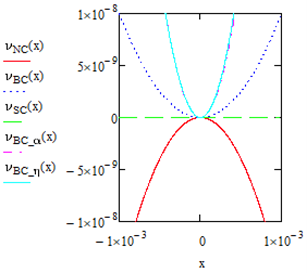
\includegraphics[width=\linewidth]{YVSbypass_nu_x}
  \end{panel}\hfill
  \begin{panel}{0.32\textwidth}
    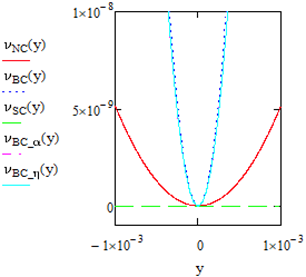
\includegraphics[width=\linewidth]{YVSbypass_nu_y}
  \end{panel}\hfill
  \begin{panel}{0.32\textwidth}
    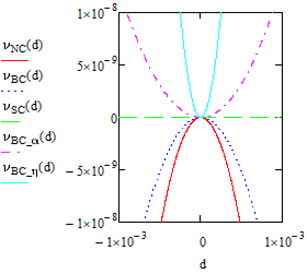
\includegraphics[width=\linewidth]{YVSbypass_nu_d}
  \end{panel}
  \caption{Spin precession frequency versus the coordinates $x$ (a), $y$ (b) and
    $\delta$ (c) for different optimization cases: NC, natural chromaticity
    (red); BC, zero betatron chromaticity (blue dotted); SC, spin coherence
    (green); BC$_\alpha$, zero chromaticity and $\alpha_1=0$ (violet);
    BC$_\eta$, zero chromaticity and $\eta_1 = 0$ (light blue).}
  \label{fig:bypass_nu}
\end{figure}

\begin{table}[htbp]
  \centering
  \caption{Main parameters of the NICA ring with bypasses for different
    optimization cases. $K_x$, $K_y$, $K_z$ are the coefficients of the
    quadratic terms of the spin precession frequency in $x$, $y$ and $\delta$.}
  \label{tab:bypass_opt}
  \small
  \setlength{\tabcolsep}{3pt}
  \begin{tabular}{lcccc}
    \toprule
    Optimization & None & Chromaticity & \makecell{Spin\\coherence}
      & \makecell{Chromaticity\\$+\,\eta_1$} \\
    \midrule
    Chromaticity $\xi_x/\xi_y$ & $-17/{-17}$ & $0/0$ & $-13/{-18}$ & $0/0$ \\
    $\alpha_1$ & 0.2 & $-0.4$ & $-0.37\times10^{-2}$ & $-0.85$ \\
    $K_x$ & $-0.16\times10^{-1}$ & $0.55\times10^{-1}$ & $0.27\times10^{-13}$ & $0.56\times10^{-1}$ \\
    $K_y$ & $0.51\times10^{-2}$ & $0.76\times10^{-1}$ & $-0.12\times10^{-12}$ & $0.78\times10^{-1}$ \\
    $K_z$ & $-0.43\times10^{-1}$ & $0.20\times10^{-1}$ & $0.13\times10^{-12}$ & $1.6\times10^{-1}$ \\
    Sextupole families & none & 2 & 3 & 3 \\
    \makecell[l]{Max.\ sextupole\\strength, m$^{-3}$} & -- & 2.7 & 19.4 & 104.2 \\
    \bottomrule
  \end{tabular}
\end{table}

\subsection{Conclusion}

For EDM experiments it is necessary to use NICA as a storage ring. For this
reason, a modernization was considered by creation of alternative straight
sections parallel to the original ones by using bypass channels. Also, the
straight sections have the ability to place special elements---Wien
filters---to compensate the spin rotation in the arcs. As the arcs remain
unchanged, this allows one to use NICA in various experiments.

Two principal schemes of the bypass channel were considered, and finally the
most realistic case was obtained, where the straight section is fully regular.
The final structure satisfies all necessary magneto-optics requirements.
Spin-tracking research with optimized Wien filters was made, and simulations
show that the spin restores its orientation at the straight sections. The
quasi-frozen spin method can be implemented in bypass NICA.

The material of this section has been reported
in~\cite{Senichev:2022ide,Kolokolchikov:2023cla,Kolokolchikov:2023zpy,Kolokolchikov:2023zhf,Aksentev:2022boh,Aksentev:2023xnd,Melnikov:2023_jetpl_decoherence,Melnikov:2024gcc,Aksentev:2024tmx,Senichev:2024qtr,Senichev:2025jqf}.

% ===== 04-nuclotron =====
\section{Modernized Nuclotron}
\label{sec:nuclotron}

\subsection{Present Nuclotron lattice}

Figure~\ref{fig:nica_complex} shows the NICA accelerator complex, which
comprises the Booster, the Nuclotron and the Collider. The Booster and the
Nuclotron serve as the injector of heavy ions, polarized protons and
deuterons into the collider. The Nuclotron lattice was originally designed to
be as close to circular as possible and has eight superperiods.
Figure~\ref{fig:nuclotron_twiss} shows the Twiss functions of one superperiod,
which consists of a bending arc of three FODO cells, each with four bending
magnets with a maximum field of \SI{1.8}{T}, and a straight section of one FODO
cell. The Nuclotron circumference is \SI{251}{m}.

\begin{figure}[htbp]
  \centering
  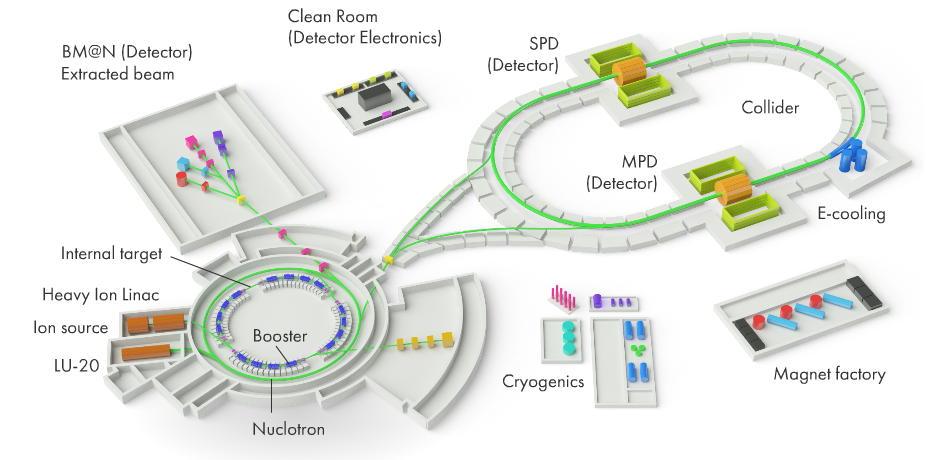
\includegraphics[width=0.85\textwidth]{YVScomplexNICA}
  \caption{NICA accelerator complex.}
  \label{fig:nica_complex}
\end{figure}

\begin{figure}[htbp]
  \centering
  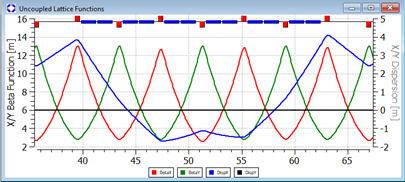
\includegraphics[width=0.7\textwidth]{YVSnuclotron_twiss}
  \caption{Twiss functions of one Nuclotron superperiod.}
  \label{fig:nuclotron_twiss}
\end{figure}

The main drawback of the Nuclotron, both as a collider injector and as a
stand-alone ring, is the limited length of the drift spaces in which the
equipment for these two functions must be installed. All modernization options below
are assessed with respect to this limitation.

\subsection{Modernization options}

Two modernization options of the Nuclotron have been studied. The adaptation of
the Nuclotron magneto-optical structure to the deuteron (and proton) EDM search
in the quasi-frozen spin regime is developed
in~\cite{Senichev:2023vtx,Senichev:2024vhw,Senichev:2025ude,Senichev:2026xca}.

The first option, Nuclotron~2.1, is a lattice that preserves all properties of
the existing accelerator and allows deuteron EDM experiments with electric
deflectors or Wien filters installed in the ring. Either device keeps the spin
of the polarized beam along its direction of motion around the ring. Within the
eight-superperiod lattice, $N_{super} = 8$, this requires implementing the
frozen (or quasi-frozen) spin concept by lengthening the straight sections
between the arcs, ensuring zero dispersion in the straight sections, and, if
possible, keeping the ring circumference so that the equipment fits into the
existing tunnel~\cite{Senichev:2023vtx,Senichev:2024vhw}. An axion search could also be included in this framework,
although the treatment of the systematic errors of such an experiment is not
yet fully understood. In the Nuclotron~2.1 option, all key collider
parameters, such as the transition energy and the electron cooler parameters,
remain unchanged. This creates a serious problem at the interface between the
collider and the Nuclotron: crossing the transition energy with a cooled beam
leads to irreversible beam degradation and a lower final luminosity.

The Nuclotron~2.2 option introduces modifications that ensure compatibility
with the collider. The injection energy of polarized protons into the collider
remains at 2--\SI{3}{GeV}. To eliminate the effect of transition crossing after
electron cooling, the transition energy of the collider is to be raised above
its maximum operating energy. In addition, a lower maximum energy of heavy ions
and polarized particles in Nuclotron~2.2 is considered. This frees space in the
ring for Wien filters and extends the capabilities of the Nuclotron for EDM and
axion experiments. A lower Nuclotron energy does not degrade the complex as a
whole, since the collider can take over some functions of the Nuclotron and
provide proton and heavy-ion beams over the entire Nuclotron energy range.

\subsection{Nuclotron 2.1: quasi-frozen spin for deuterons}

Adapting the Nuclotron lattice to the measurement of the deuteron EDM involves
three problems: lengthening the straight sections, suppressing the dispersion
in the straight sections, and keeping the spin direction along the momentum
around the ring.

The first problem is solved by raising the maximum field of the bending
magnets to \SI{1.8}{T} and by merging the two adjacent magnets between the
quadrupoles into one magnet. At the same time, the dispersion is suppressed by
choosing the horizontal phase advance in the arcs. One superperiod of the
modernized Nuclotron~2.1 is shown in Fig.~\ref{fig:nuclotron21}. The main
parameters of Nuclotron~2.1 are: circumference \SI{251}{m}; betatron tunes
$Q_x = 9.78548$, $Q_y = 10.6839$; momentum compaction factor 0.0134394; slip
factor $-0.0222388$; natural chromaticity $-16.0394$ (horizontal) and
$-17.8984$ (vertical). In the figure, D denotes a defocusing quadrupole, F a
focusing quadrupole, B a dipole magnet and ED an electrostatic deflector. The
parameters of all options are summarized in Table~\ref{tab:nuclotron}.

\begin{figure}[htbp]
  \centering
  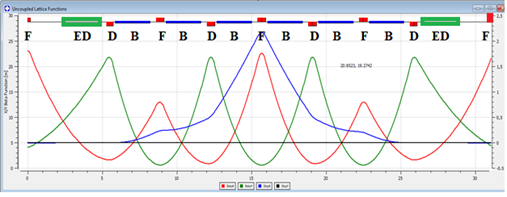
\includegraphics[width=0.8\textwidth]{YVSnuclotron21_twiss}
  \caption{Twiss functions of one superperiod of the modernized Nuclotron~2.1
    with two electrostatic deflectors.}
  \label{fig:nuclotron21}
\end{figure}

With the bending field raised to \SI{1.8}{T}, the length of the straight
section in each superperiod increases from 7.3 to \SI{10.5}{m}. The third
problem, keeping the spin direction relative to the momentum as required for
the detection of the deuteron EDM signal, is solved with negative-curvature
electrostatic deflectors in each superperiod (Fig.~\ref{fig:nuclotron_ed}).

In the quasi-frozen spin concept, the magnetic and electric fields act in
different elements. The spin direction therefore oscillates relative to the
direction of motion, since the spin rotates in opposite directions in the
magnetic and electrostatic bending elements. The deuteron magnetic anomaly is
small, $G = -0.143$. The spin oscillates around the momentum in each magnetic
arc within half of the spin phase advance,
$\Phi_s = \frac{1}{2N}\,2\pi\gamma G$, and each time it is turned back by
$-\Phi_s$ in the electrostatic deflector; here $N$ is the arc superperiodicity.
This keeps the average spin direction along the momentum around the whole ring,
in accordance with the quasi-frozen spin concept~\cite{Senichev:2020_qfs_features}.

For the Nuclotron, $N = 8$. Owing to the small value of $\Phi_s$, the effective
EDM signal is reduced only by the factor
\begin{equation}
  J_0(\Phi_s) \approx 1 - \frac{\Phi_s^2}{4},
\end{equation}
i.e., by a few percent at most.

To determine the parameters of the electrostatic deflectors in the
quasi-frozen spin mode for deuterons, consider the lattice as consisting of
two different parts (Fig.~\ref{fig:nuclotron_ed}). The magnetic arcs bend the
beam by $\Phi^B = 2\pi/N + 2\alpha$ each and rotate the spin in the horizontal
plane relative to the momentum by $\Phi^B_s = \nu^B_s\Phi^B$. The electrostatic
arcs with negative-curvature deflectors bend the beam by $\Phi^E = -2\alpha$
each and rotate the spin relative to the momentum in the opposite direction by
$\Phi^E_s = \nu^E_s\Phi^E$. The quasi-frozen spin condition requires
$\Phi^E_s = -\Phi^B_s$. Since in an electrostatic deflector the spin rotates
relative to the momentum many times faster than in a magnetic field, the two
types of arcs are related by
\begin{equation}
  \nu_s^B\left(\frac{2\pi}{N}+2\alpha\right) = \nu_s^E\, 2\alpha,
  \qquad
  \alpha = \frac{1}{\nu_s^E/\nu_s^B-1}\,\frac{\pi}{N} = -\gamma^2\frac{G}{G+1}\,\frac{\pi}{N},
  \label{eq:nuclotron_alpha}
\end{equation}
where $\nu_s^E$ and $\nu_s^B$ are given by Eqs.~\eqref{eq:nu_e}
and~\eqref{eq:nu_b}. For given bending magnets and a deflector field
$E_{ED} = \SI{130}{kV/cm}$, one obtains $\nu_s^E/\nu_s^B$, the parameter
$\alpha$ and the radius of curvature of the deflector $R_{ED} = \kappa/E_{ED}$,
where $\kappa = p_0\beta c/e$ is the electric rigidity and
$p_0 = \gamma m\beta c$, so that
$R_{ED} = \frac{mc^2}{e}\frac{\gamma\beta^2}{E_{ED}}$. The deflector length is
then
$L_{ED} = 2\alpha R_{ED} = -2\frac{\gamma^2 G}{G+1}\frac{\pi}{N}R_{ED}$.
Figure~\ref{fig:nuclotron_ed} shows how the electrostatic deflectors are
inserted to realize the quasi-frozen spin lattice of the Nuclotron. At the
optimal polarimeter energy $W = \SI{270}{MeV}$~\cite{Kurilkin:2010ym},
$\alpha = 0.026\pi$ and the required length of the electrostatic channel is
\SI{7.3}{m}. The EDM signal relative to the frozen spin case,
$S^{QFS}_{EDM}/S^{FS}_{EDM} = 1-\alpha^2/4 \approx 0.998$, is reduced by only
0.2\%.

The electrostatic arc with negative curvature leaves room for the necessary
equipment in the straight section between two magnetic arcs; when the
electrostatic deflectors are switched off, the beam passes straight through
this section.

\begin{figure}[htbp]
  \centering
  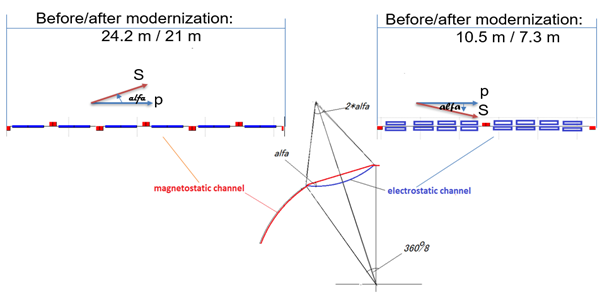
\includegraphics[width=0.8\textwidth]{YVSnuclotron_ed_insert}
  \caption{Electrostatic insertion compensating the spin rotation in the
    magnetic arc.}
  \label{fig:nuclotron_ed}
\end{figure}

A lattice with twice the number of superperiods, 16, was also considered.
By splitting the double bending magnets into individual magnets, the number of
FODO cells per superperiod is doubled, and with a \ang{60} phase advance per
FODO cell the dispersion is suppressed in every second straight section. In
this version $\alpha = 0.013\pi$, and the EDM signal relative to the frozen spin
case is $1-\alpha^2/4 \approx 0.9996$, i.e., reduced by only 0.04\%, which makes
this lattice practically equivalent to the frozen spin one. This lattice can
also be used for the proton EDM, since the spin rotation angle of protons in
the magnetic arcs is only about \ang{30}.

\subsection{Nuclotron 2.2: quasi-frozen spin with Wien filters for deuterons}

In the Nuclotron~2.2 lattice, a small vertical magnetic field of about
\SI{100}{mT} is added to compensate the Lorentz force of the electric field,
so that the electrostatic deflectors become straight. With the magnetic field
added, the E+B element is a Wien filter. The ring then consists of arcs
connected by straight sections with Wien filters, in which crossed electric
and magnetic fields keep the particles on a straight path (zero Lorentz force)
and compensate the spin rotation accumulated in the magnetic arcs. The total
length of the Wien filters is determined by the beam parameters and by the
required compensation of the spin rotation in the arcs, whereas their number
is chosen for convenient placement around the ring.

With $N$ magnetic arcs in total, each arc bends the particles by
$\Phi^B_{arc} = 2\pi/N$ and rotates the spin in the horizontal plane relative
to the momentum by $\Phi^{arc}_s = \gamma G\,\Phi^B_{arc}$. The Wien filters
rotate the spin relative to the momentum in the opposite direction. In the
electric field $E_{wf}$ the spin rotation angle is
\begin{equation}
  \Phi^E_{swf} = -\left(\gamma G+\frac{\gamma}{\gamma+1}\right)\beta^2\,\Phi^E_{wf},
\end{equation}
where $\Phi^E_{wf} = \frac{eE_{wf}}{m_0c^2\gamma\beta^2}L_{wf}$ is the momentum
rotation angle in the electric field of the Wien filter, and in the magnetic
field $B_{wf}$ it is
\begin{equation}
  \Phi^B_{swf} = (\gamma G+1)\,\Phi^B_{wf},
\end{equation}
where $\Phi^B_{wf} = \frac{eB_{wf}}{m_0c\gamma\beta}L_{wf}$ is the momentum
rotation angle in the magnetic field of a Wien filter of length $L_{wf}$.

Since the Lorentz force in the Wien filter vanishes, the angles must be equal,
$\Phi^E_{wf} = \Phi^B_{wf}$, and they can be expressed through the electric
field $E_{wf}$ and the length $L_{wf}$ of the filters installed in all $N$
straight sections. In the frozen spin option, the total spin precession
frequency relative to the momentum in the combined E+B bending element is
zero. The quasi-frozen spin option instead requires the total spin rotation
angle per turn in the E and B fields to vanish. The QFS condition therefore
reads
\begin{equation}
  (\gamma G+1)\,\Phi^B_{wf} - \left(\gamma G+\frac{\gamma}{\gamma+1}\right)\beta^2\,\Phi^E_{wf} = \gamma G\,\frac{2\pi}{N},
\end{equation}
which gives the parameters of one Wien filter:
\begin{equation}
  L_{wf}E_{wf} = \frac{2\pi}{N}\,\frac{G}{G+1}\,\frac{m_0c^2}{e}\,\beta^2\gamma^3,
  \qquad
  B_{wf} = -\frac{E_{wf}}{c\beta},
  \label{eq:nuclotron_wf}
\end{equation}
where $L_{wf}$ is the length of one Wien filter. The total length of all Wien
filters,
$L^\Sigma_{wf}E_{wf} = 2\pi\frac{G}{G+1}\frac{m_0c^2}{e}\beta^2\gamma^3$,
depends only on the particle species and energy.

Equations~\eqref{eq:nuclotron_alpha} and~\eqref{eq:nuclotron_wf}, derived for
electrostatic deflectors and for Wien filters, show that the type of the
compensating element does not matter. With the magnetic arc unchanged, the
Wien filters are shorter by the total length of the kickers, since a Wien filter
combines the functions of an electrostatic deflector and a kicker in one
element.

Figure~\ref{fig:nuclotron221} shows the Twiss functions of one superperiod of
the first version of the modernized lattice, Nuclotron~2.2.1. Two Wien filters
installed in the central straight sections of the superperiod restore the spin
direction after each magnetic half-arc. The spin deviation angle from the
momentum, $\alpha = \gamma G\,2\pi/N$, characterizes how much the quasi-frozen
spin lattice differs from the frozen spin one. In this lattice, the number of
arcs that determine the spin deviation equals the number of superperiods,
$N = 8$.

\begin{figure}[htbp]
  \centering
  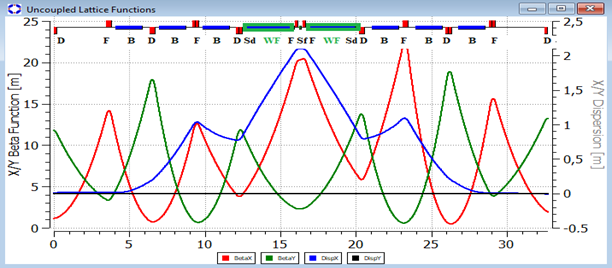
\includegraphics[width=0.8\textwidth]{YVSnuclotron221_twiss}
  \caption{Twiss functions of one superperiod of the modernized
    Nuclotron~2.2.1 with two Wien filters.}
  \label{fig:nuclotron221}
\end{figure}

For a maximum electric field of \SI{130}{kV/cm}, the magnetic field is below
\SI{80}{mT}. Such a low magnetic field simplifies the Wien filter design: a
permanent magnet or an air-core coil can be used. For these fields and a
deuteron energy of \SI{270}{MeV}, the total length of the Wien filters in all
straight sections is about \SI{52}{m}, and the length of one Wien filter is
\SI{3.25}{m}. At \SI{270}{MeV} (\SI{135}{MeV} per nucleon), the maximum spin
deviation is $\alpha\sim\pm\ang{3}$ over one arc, which is a good
approximation to a regular frozen spin lattice.

In the next version, Nuclotron~2.2.2, the Wien filters are distributed over
four straight sections of the superperiod (Fig.~\ref{fig:nuclotron222}). Each
arc of the superperiod is thus split into two arcs, and with respect to the
bending magnets the lattice has the superperiodicity $N = 16$, while the overall
superperiodicity of the lattice with all elements remains 8. This solves two
problems. First, the ring becomes a 16-sided polygon, i.e., closer to a circle,
and fits the existing tunnel better. Second, with a bending magnet length of
\SI{1.77}{m} and a Wien filter length of \SI{1.65}{m}, the spin deviation is
$\alpha\sim\pm\ang{1.5}$, half that of version~2.2.1. This brings the
properties of the quasi-frozen spin lattice much closer to those of the frozen
spin lattice.

\begin{figure}[htbp]
  \centering
  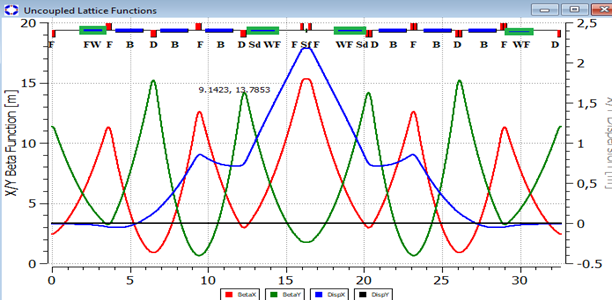
\includegraphics[width=0.8\textwidth]{YVSnuclotron222_twiss}
  \caption{Twiss functions of one superperiod of the modernized
    Nuclotron~2.2.2 with four Wien filters.}
  \label{fig:nuclotron222}
\end{figure}

To increase the energy, the modification Nuclotron~2.2.3 with fewer empty
drift spaces and longer magnets was considered (Fig.~\ref{fig:nuclotron223}).
In this lattice, the maximum energy is \SI{3.5}{GeV} per nucleon for deuterons
and \SI{7.8}{GeV} for protons, which is much closer to the present Nuclotron.

\begin{figure}[htbp]
  \centering
  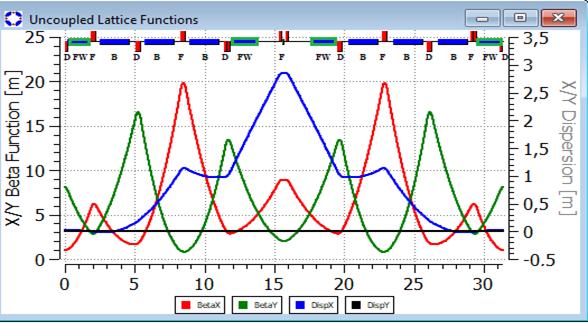
\includegraphics[width=0.75\textwidth]{YVSnuclotron223_twiss}
  \caption{Twiss functions of one superperiod of the modernized
    Nuclotron~2.2.3 with four Wien filters.}
  \label{fig:nuclotron223}
\end{figure}

\begin{table}[htbp]
  \centering
  \caption{Main parameters of the Nuclotron modifications.}
  \label{tab:nuclotron}
  \footnotesize
  \setlength{\tabcolsep}{2.5pt}
  \begin{tabular}{lcccccccc}
    \toprule
    \makecell[l]{Nuclotron\\lattice} & \makecell{Magnet\\length, m} & \makecell{Number of\\magnets}
      & \makecell{Total magnet\\length, m} & \makecell{$B_{max}$,\\T}
      & \makecell{$B_{max}R$,\\T$\cdot$m} & \makecell{$W_d^{max}$,\\GeV}
      & \makecell{$W_d^{max}$,\\GeV/u} & \makecell{$W_p^{max}$,\\GeV} \\
    \midrule
    Present & 1.44 & 96 & 138.24 & 1.8 & 39.6  & 10.14 & 5.07 & 10.97 \\
    2.1     & 2.35 & 48 & 112.77 & 1.8 & 32.2  & 8     & 4    & 8.79 \\
    2.2.1   & 1.78 & 48 & 85.3   & 1.8 & 24.4  & 5.7   & 2.85 & 6.47 \\
    2.2.2   & 1.78 & 48 & 85.44  & 1.8 & 24.5  & 5.7   & 2.85 & 6.47 \\
    2.2.3   & 2.10 & 48 & 101    & 1.8 & 28.93 & 7.0   & 3.5  & 7.8 \\
    \bottomrule
  \end{tabular}
\end{table}

\subsection{Nuclotron 2.2.2: quasi-frozen spin with Wien filters for protons}

With a magnetic superperiodicity of 16, the lattice can also be used for
protons at a reduced energy. The energy is then limited mainly by the free
space for the Wien filters, which is \SI{52}{m} in this lattice. The maximum
proton energy follows from Eq.~\eqref{eq:nuclotron_wf}:
\begin{equation}
  \gamma(\gamma^2-1) = L_{wf}\,\frac{eE_{wf}}{mc^2}\,\frac{N}{2\pi}\,\frac{G_p+1}{G_p},
\end{equation}
where $L_{wf}N = \SI{52}{m}$ and $G_p = 1.793$ is the proton magnetic anomaly.
Solving for $\gamma$ gives $\gamma = 1.08047$, i.e., $W_p\approx\SI{80}{MeV}$.
At this energy, the spin deviation in a magnetic arc is determined by
$\gamma G_p = 1.93711$, and the spin deviation angle is
$\alpha = \pm\frac{1}{2}\frac{\gamma G_p}{16}$, which amounts to
$\alpha = \ang{3.5}$.
The same lattice as for deuterons can be used for protons, but at a lower
energy and with the Wien filters rotated by \ang{180}, since the magnetic
anomalies of the two particles have opposite signs. At a proton energy of
\SI{80}{MeV} the lattice thus behaves practically as a frozen spin lattice.
Figure~\ref{fig:pc_ay} shows the p--C analyzing power in terms of the
``average analyzing power'' taken from Ref.~\cite{Mcnaughton:1985wyt}.

\begin{figure}[htbp]
  \centering
  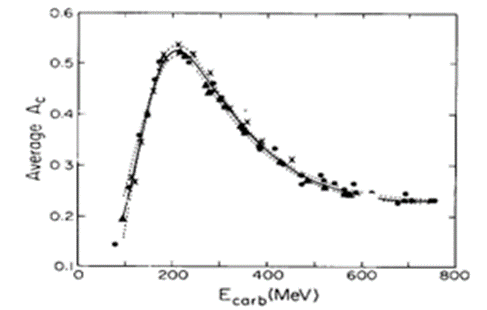
\includegraphics[width=0.6\textwidth]{YVSpc_analyzing_power}
  \caption{Average p--C analyzing power $\overline{A_c}$ for
    $\theta_{lab} = \ang{5}$--\ang{20} at discrete energies (points) and its
    continuous energy dependence (solid line). The data are from SIN
    ($\triangle$), TRIUMF ($\times$) and LAMPF ($\bullet$)~\cite{Mcnaughton:1985wyt}.}
  \label{fig:pc_ay}
\end{figure}

Figure~\ref{fig:pc_ay} shows that the analyzing power near \SI{100}{MeV} is
about 0.2, i.e., 0.35 of its maximum value $A_c = 0.53$ at \SI{230}{MeV}. This
makes proton EDM studies at this energy in the Nuclotron~2.2.2 lattice
feasible in parallel with full-scale deuteron measurements.

Galactic axions can be searched for with the same equipment as the EDM.
Varying the spin precession frequency at a fixed beam energy turns the booster
with Wien filters into a broadband antenna that searches for axions through a
resonant full or partial spin flip in the oscillating pseudomagnetic field of
the axion halo of our Galaxy~\cite{Nikolaev:2022wyi}. The growth of the
horizontal polarization induced by axions is extracted by a Fourier analysis of
the oscillating vertical asymmetry in the internal
polarimeter~\cite{JEDI:2015vwa}.

\subsection{Maximum energy of heavy ions and protons in Nuclotron 2.2.2}

The calculations show that deuteron and proton EDM experiments in the
Nuclotron~2.2.2 lattice require free space for Wien filters with a total length
of \SI{52}{m}. With the tunnel circumference fixed at \SI{251}{m}, this is
possible either by raising the field of the bending magnets, which is already
set to \SI{1.8}{T}, or by reducing their total length. Assuming that the
bending field does not exceed \SI{1.8}{T}, the second option was chosen, which
inevitably lowers the maximum particle energy in the Nuclotron.

\subsection{Features of the modernized Nuclotron lattice}

The lattice of the modernized Nuclotron was designed with several goals.
First, the superperiod has a drift without bending magnets in its central
cell, where the dispersion function reaches its maximum and the orbit
curvature is zero ($\rho\to\infty$). This makes it possible to raise the
transition energy, since the momentum compaction factor is
\begin{equation}
  \alpha = \frac{1}{C}\oint\frac{D(s)}{\rho(s)}\,ds .
\end{equation}
Second, the number of superperiods $s = 8$ is only slightly larger than the
horizontal betatron tune $\nu_x$, which makes the momentum compaction factor
easy to adjust, as in the resonant lattices with a low or negative momentum
compaction factor~\cite{Senichev:1997kn,Ishi:1998tj,Papaphilippou:2010zz,Senichev:2008zza,Toelle:2007zz}:
\begin{equation}
  \alpha = \frac{\nu_x^3}{R}\sum_{k=0}^{\infty}\frac{a_k^2}{\nu_x^2-(ks)^2},
\end{equation}
where $a_k$ are the harmonics of the dispersion-generating perturbation.
Third, the central drift simplifies the placement of the three sextupole
families needed to control the betatron and spin chromaticities, whereas the
side drifts are convenient for the Wien filters. Finally, the maximum of the
dispersion at the center of the superperiod coincides with the minimum of the
horizontal beta function $\beta_x$.

The material of this section has been reported
in~\cite{Senichev:2023vtx,Senichev:2024vhw,Senichev:2024fey,Senichev:2025ude,Senichev:2026xca,Kolokolchikov:2025sew,Senichev:2025jqf}.

% ===== 05-specialized-ring =====
\section{Specialized frozen spin rings at JINR}
\label{sec:specialized-ring}

This section presents two specialized frozen spin lattices designed
exclusively for the search for the electric dipole moments of the proton and
the deuteron: an all-electrostatic ring for protons and a ring with combined
E+B deflectors for deuterons~\cite{Palamarchuka:2026pyv}.

\subsection{Frozen spin option for the proton beam}

The frozen spin lattice for a proton beam is the simplest one in terms of
parameter choice and is uniquely defined. It consists of electrostatic
deflectors whose total length $L_{total}$ is determined by the beam energy and
the maximum permissible electrostatic field strength:
\begin{equation}
  L_{total} = 2\pi\,\frac{mc^2}{eE}\,\gamma\beta^2 .
  \label{eq:pring_length}
\end{equation}
For an energy of \SI{233}{MeV} and a maximum field of $E = \SI{120}{kV/cm}$,
the total length of all electrostatic deflectors is $L_{total} = \SI{219.55}{m}$.

With 50 deflectors placed around the ring, the length of a single deflector is
$L_{def} = \SI{4.39}{m}$. The 50 deflectors are divided into five groups, each
consisting of five FODO cells and containing ten deflectors
(Fig.~\ref{fig:pring_superperiod}).

\begin{figure}[htbp]
  \centering
  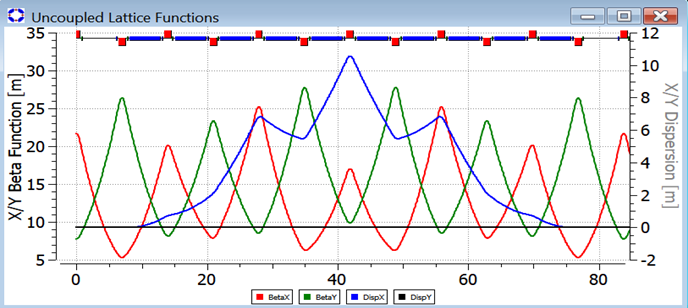
\includegraphics[width=0.8\textwidth]{YVSpring_superperiod}
  \caption{Twiss functions of one superperiod of the electrostatic proton
    ring.}
  \label{fig:pring_superperiod}
\end{figure}

Figure~\ref{fig:pring_twiss} shows the whole ring, which consists of five
superperiods. Each superperiod comprises an achromat with drift spaces at both
ends, so that the phase advance per superperiod is not an integer multiple of
$2\pi$. The ring circumference is \SI{419.1}{m}. The layout of the
electrostatic ring is shown in Fig.~\ref{fig:pring_layout}; it closely
resembles a circle.

\begin{figure}[htbp]
  \centering
  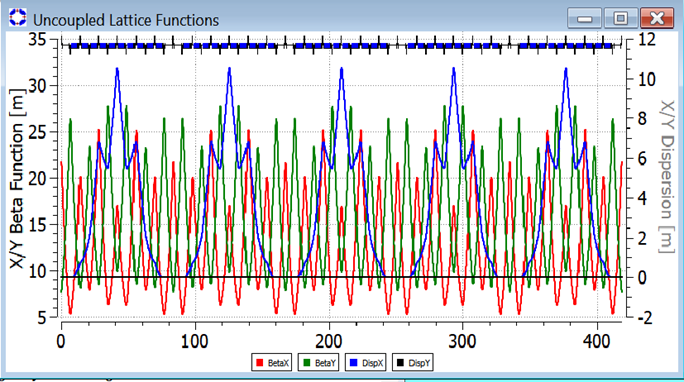
\includegraphics[width=0.8\textwidth]{YVSpring_twiss}
  \caption{Twiss functions along the whole electrostatic proton ring.}
  \label{fig:pring_twiss}
\end{figure}

\begin{figure}[htbp]
  \centering
  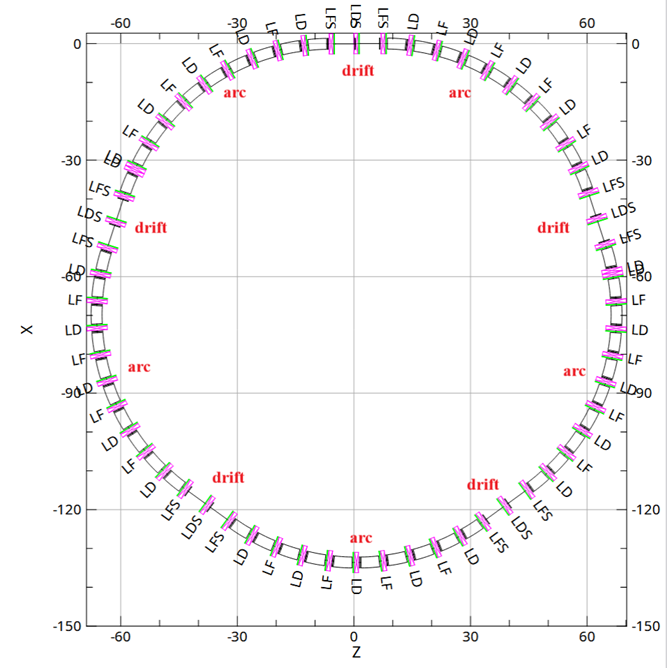
\includegraphics[width=0.6\textwidth]{YVSpring_layout}
  \caption{Layout of the electrostatic proton ring.}
  \label{fig:pring_layout}
\end{figure}

Tables~\ref{tab:pring} and~\ref{tab:pring-cont} summarize the ring parameters
required to estimate its dimensions and cost.

\begin{table}[!htbp]
  \caption{Parameters of the frozen spin electrostatic ring for the proton
    EDM search.}
  \label{tab:pring}
  \centering
  \renewcommand{\baselinestretch}{1}\small\selectfont
  \begin{tabular}{@{}p{0.60\linewidth}@{\hspace{1em}}p{0.32\linewidth}@{}}
    \toprule
    Parameter & Value \\
    \midrule
    Circumference, m & 419.1 \\
    Symmetry order (number of arcs and straight sections) & 5 \\
    Injection energy, MeV & 20 \\
    Proton magnetic anomaly $G$ & 1.793 \\
    Final energy, MeV & 233.8 \\
    EDM experiment energy, MeV & 233.8 \\
    Initial and final relative velocity and Lorentz factor
      & $\beta=0.2$, $\gamma=1.0213$; $\beta=0.6$, $\gamma=1.248$ \\
    Revolution frequency at the beginning and end of the cycle, MHz
      & 0.143--0.429 \\
    Harmonic number & 20 \\
    RF frequency at the beginning and end of the cycle, MHz & 2.8--8.6 \\
    \bottomrule
  \end{tabular}
\end{table}

\begin{table}[!htbp]
  \caption{Parameters of the frozen spin electrostatic ring for the proton
    EDM search (continued).}
  \label{tab:pring-cont}
  \centering
  \renewcommand{\baselinestretch}{1}\small\selectfont
  \begin{tabular}{@{}p{0.60\linewidth}@{\hspace{1em}}p{0.32\linewidth}@{}}
    \toprule
    Parameter & Value \\
    \midrule
    \multicolumn{2}{c}{\textbf{Arcs}} \\
    \midrule
    Arc length, m & 70.1 \\
    Arc superperiodicity & regular lattice \\
    Arc lattice & 5 FODO cells \\
    Number of electrostatic deflectors per arc & 10 \\
    Deflector length, m & 4.39 \\
    Deflector type & cylindrical \\
    Maximum electric field of the deflector, MV/m & 12 \\
    Number of quadrupoles per arc & 9 + 1 (two end halves) \\
    Quadrupole type & electrostatic \\
    Quadrupole families & one focusing (LF), one defocusing (LD) \\
    Maximum quadrupole gradient in the arcs, kV/cm$^2$
      & LF $= 6.78$, LD $= -6.18$ \\
    Quadrupole length, m & 1.0 \\
    Number of chromatic sextupoles per arc & 10 \\
    Sextupole type & electric or magnetic \\
    Sextupole strengths & to be determined \\
    Betatron tunes $\nu_x/\nu_y$ & 6.12/4.72 (preliminary) \\
    Natural chromaticity $\xi_x/\xi_y$ & to be determined \\
    Transition energy, GeV & 3.1 \\
    Maximum $\beta_x/\beta_y$, m & 27.9/34.8 \\
    Maximum horizontal dispersion, m & 10.8 \\
    \midrule
    \multicolumn{2}{c}{\textbf{Straight sections between arcs}} \\
    \midrule
    Length of straight sections, m & $5\times 13.5$ \\
    Lattice of straight sections & DOFFOD \\
    Quadrupole gradients, T/m & QF $= 7.93$, QD $= -7.11$ \\
    Drift length between adjacent quadrupoles, m & 6.0 \\
    \bottomrule
  \end{tabular}
\end{table}

As a second option, a racetrack ring with two arcs and dispersion suppressors
at both ends of each arc was considered (Fig.~\ref{fig:pring_suppressor}). One
of the two options will be adopted in the course of further lattice
development, which will take spin decoherence into
account~\cite{Senichev:2013dra}.

\begin{figure}[htbp]
  \centering
  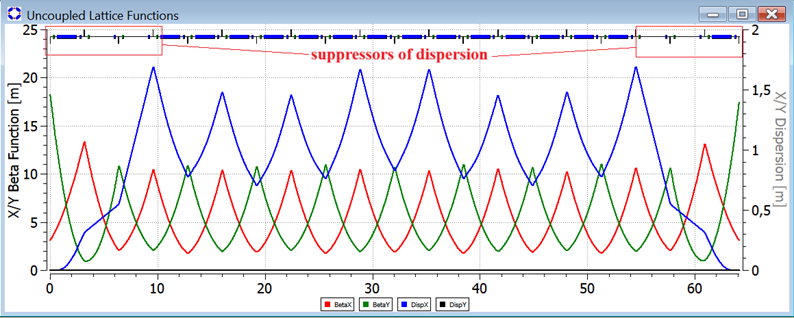
\includegraphics[width=0.9\textwidth]{YVSpring_arc_suppressor}
  \caption{Arc with dispersion suppressors at both ends (racetrack option of
    the proton ring).}
  \label{fig:pring_suppressor}
\end{figure}

\subsection{Frozen spin option for the deuteron beam}

The frozen spin lattice for a deuteron beam differs from the proton one in the
composition of the equipment and in the elements used. Here the bending
deflector with E+B fields consists of electrostatic plates
generating a horizontal electric field, inserted into the gap of a dipole
magnet with a vertical magnetic field (Fig.~\ref{fig:dring_deflector}).

\begin{figure}[htbp]
  \centering
  \begin{panel}[b]{0.38\textwidth}
    \centering
    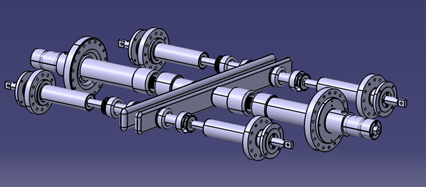
\includegraphics[width=\textwidth]{YVSdring_deflector}
  \end{panel}
  \hfill
  \begin{panel}[b]{0.58\textwidth}
    \centering
    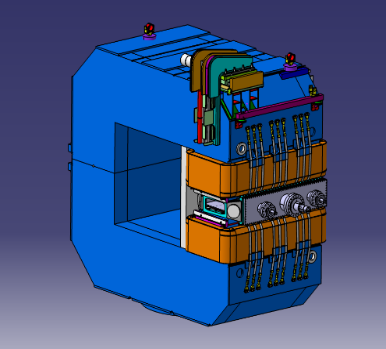
\includegraphics[width=\textwidth]{YVSdring_magnet}
  \end{panel}
  \caption{Electrostatic deflector (a) and vertical-field dipole magnet with
    the electrostatic deflector inserted into its gap (b).}
  \label{fig:dring_deflector}
\end{figure}

The condition of stable motion on an orbit of radius $R$ follows from the
balance of the Lorentz and centrifugal forces:
\begin{equation}
  R = \frac{\gamma m_0 v^2}{e\left|\vec E + c\vec\beta\times\vec B\right|},
  \label{eq:dring_radius}
\end{equation}
from which the momentum precession frequency in the combined fields is
\begin{equation}
  \vec\Omega_p = \frac{e\vec E}{m_0\gamma\beta c} + \frac{e\,c\vec\beta\times\vec B}{m_0\gamma\beta c}.
\end{equation}
Subtracting $\vec\Omega_p$ from $\vec\Omega_{mdm}$ gives the spin precession
frequency relative to the momentum:
\begin{equation}
  \vec\Omega^{p}_{mdm} = \frac{e}{m_0\gamma}\left\{\gamma G\vec B
    + \left(\frac{1}{\gamma^2-1} - G\right)\frac{\vec\beta\times\vec E}{c}\right\}.
\end{equation}

A frozen spin lattice for EDM studies has to satisfy two conditions. The first
relates the external fields to the orbit radius, Eq.~\eqref{eq:dring_radius}
(see also~\cite{Farley:2004hp}). The second requires the spin precession
frequency relative to the direction of motion to vanish,
$\vec\Omega^{p}_{mdm} = 0$, i.e.,
$\gamma G\vec B = -\left(\frac{1}{\gamma^2-1}-G\right)\frac{\vec\beta\times\vec E}{c}$.
This fixes the relation between the fields,
\begin{equation}
  \vec E = -\frac{G\vec B c\gamma^2\beta^2}{\beta\left(1-\gamma^2\beta^2 G\right)},
\end{equation}
and the radius of curvature of the deflector,
\begin{equation}
  R = \frac{\gamma m_0 v^2}{eE\left(1-\dfrac{1}{G\gamma^2}\right)}.
\end{equation}
For an energy of \SI{270}{MeV}, the radius of curvature of the deflector is
$R = \SI{9.207}{m}$, and the total length of all deflectors is
$L_\Sigma = 2\pi R = \SI{57.85}{m}$. With 32 deflectors in total, the length of
a single deflector is $L_{def} = L_\Sigma/32 = \SI{1.808}{m}$.

Figure~\ref{fig:dring_vector} shows the vector diagram that defines the
relative directions of $\vec E$ and $\vec B$. The determining factor is the
positive vertical direction of the magnetic field, which provides the main
compensation of the centrifugal force. Since the deuteron magnetic anomaly is
negative, $G = -0.143$, the axis around which $\vec S$ precesses points
downwards. A zero precession frequency then requires the vector
$\vec\beta\times\vec E$ to point upwards, i.e., the electric field must be
directed as shown in Fig.~\ref{fig:dring_vector}.

\begin{figure}[htbp]
  \centering
  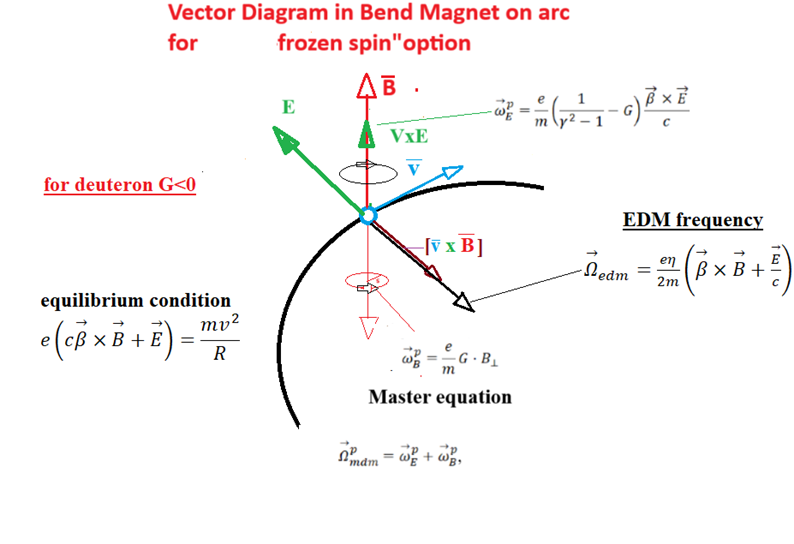
\includegraphics[width=0.75\textwidth]{YVSdring_vector_diagram}
  \caption{Vector diagram of the fields acting on a polarized deuteron.}
  \label{fig:dring_vector}
\end{figure}

Based on these relations, a frozen spin ring lattice was developed.
Figure~\ref{fig:dring_arc} shows the lattice of one arc for the deuteron beam.
The arc consists of two successive achromats with zero dispersion at its middle
and at its ends and comprises eight FODO cells.

\begin{figure}[htbp]
  \centering
  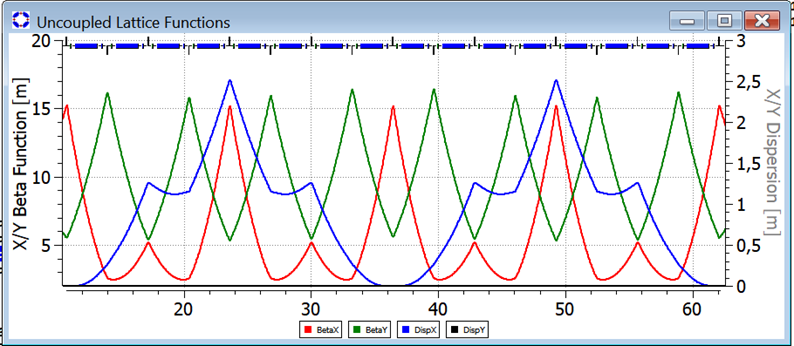
\includegraphics[width=0.85\textwidth]{YVSdring_arc_twiss}
  \caption{Twiss functions along an arc of the frozen spin deuteron ring.}
  \label{fig:dring_arc}
\end{figure}

As in the electrostatic proton ring, the dispersion modulation introduced in
the deuteron lattice provides suitable locations for sextupoles suppressing the
spin chromaticity. The main parameters of the synchrotron for the deuteron EDM
search at \SI{270}{MeV} per nucleon are listed in
Tables~\ref{tab:dring} and~\ref{tab:dring-cont}.
Figure~\ref{fig:dring_twiss} shows the Twiss functions of the whole ring with a
circumference of \SI{146}{m}; its layout is shown in
Fig.~\ref{fig:dring_layout}.

\begin{table}[!htbp]
  \caption{Parameters of the frozen spin ring with E+B
    deflectors for the deuteron EDM search.}
  \label{tab:dring}
  \centering
  \renewcommand{\baselinestretch}{1}\small\selectfont
  \begin{tabular}{@{}p{0.60\linewidth}@{\hspace{1em}}p{0.32\linewidth}@{}}
    \toprule
    Parameter & Value \\
    \midrule
    Circumference, m & 145.85 \\
    Symmetry order (number of arcs and straight sections) & 2 \\
    Injection energy, MeV/u & 40 \\
    Final energy, MeV/u & 270.0 \\
    EDM experiment energy, MeV/u & 270.0 \\
    Deuteron magnetic anomaly $G$ & $-0.143$ \\
    Initial and final relative velocity and Lorentz factor
      & $\beta=0.2$, $\gamma=1.0213$; $\beta=0.485$, $\gamma=1.143$ \\
    Revolution frequency at the beginning and end of the cycle, MHz
      & 0.143--0.99 \\
    Harmonic number $h$ & 50 \\
    RF frequency at the beginning and end of the cycle, MHz & 7.15--49.9 \\
    Length of the quarter-wave RF cavity, m & 1.502 \\
    Momentum acceptance of the separatrix at maximum energy & $1.31\times10^{-3}$ \\
    Relative momentum spread in the bunch & $5\times10^{-4}$ \\
    \bottomrule
  \end{tabular}
\end{table}

\begin{table}[!htbp]
  \caption{Parameters of the frozen spin ring with E+B
    deflectors for the deuteron EDM search (continued).}
  \label{tab:dring-cont}
  \centering
  \renewcommand{\baselinestretch}{1}\small\selectfont
  \begin{tabular}{@{}p{0.60\linewidth}@{\hspace{1em}}p{0.32\linewidth}@{}}
    \toprule
    Parameter & Value \\
    \midrule
    \multicolumn{2}{c}{\textbf{Arcs}} \\
    \midrule
    Arc length, m & 51.27 \\
    Arc superperiodicity & 2 \\
    Arc lattice & 4 + 4 FODO cells \\
    Number of E+B deflectors per arc & 16 \\
    Deflector length, m & 1.80 \\
    Deflector type & combined magnetic and electric \\
    Maximum electric field of the deflector, MV/m & 12 \\
    Number of quadrupoles per arc & 15 + 1 (two end halves) \\
    Quadrupole type & magnetic multipole \\
    Quadrupole families & one focusing (QF), one defocusing (QD) \\
    Maximum quadrupole gradient in the arcs, kG/cm
      & QF $= 1.359$, QD $= -1.00$ \\
    Quadrupole length, m & 0.1 \\
    Number of chromatic sextupoles per arc & 16 \\
    Sextupole type & magnetic \\
    Sextupole strengths, kG/cm$^2$ & SF $= 0.12$, SD $= 0.15$ \\
    Betatron tunes $\nu_x/\nu_y$ & 4.70418/2.6140 (preliminary) \\
    Natural chromaticity $\xi_x/\xi_y$ & $-4.91629/{-3.99402}$ \\
    Transition energy, GeV & 5.3 \\
    Maximum $\beta_x/\beta_y$, m & 15.1/16.5 \\
    Maximum horizontal dispersion, m & 2.5 \\
    \midrule
    \multicolumn{2}{c}{\textbf{Straight sections between arcs}} \\
    \midrule
    Length of straight sections, m & $2\times 23.3$ \\
    Lattice of straight sections & $3\times$FODO \\
    Quadrupole gradients, kG/cm & QF $= 0.734$, QD $= -0.782$ \\
    Free drift spaces between adjacent quadrupoles, m & $12\times 3.2$ \\
    \bottomrule
  \end{tabular}
\end{table}

\begin{figure}[htbp]
  \centering
  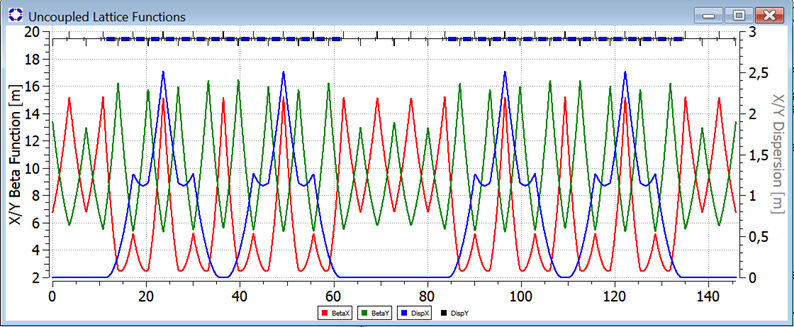
\includegraphics[width=0.85\textwidth]{YVSdring_twiss}
  \caption{Twiss functions along the frozen spin deuteron ring.}
  \label{fig:dring_twiss}
\end{figure}

\begin{figure}[htbp]
  \centering
  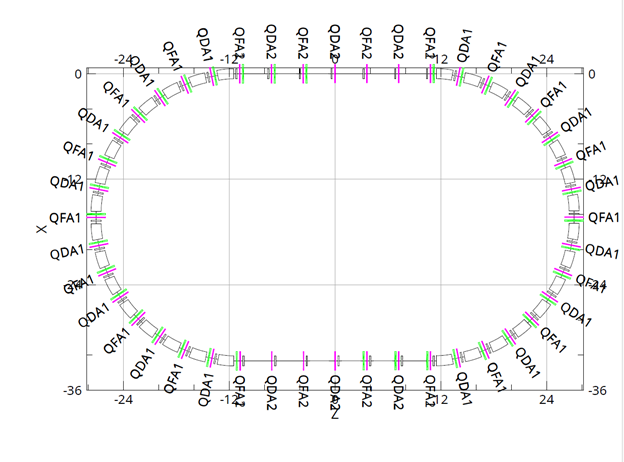
\includegraphics[width=0.75\textwidth]{YVSdring_layout}
  \caption{Layout and dimensions of the frozen spin deuteron ring.}
  \label{fig:dring_layout}
\end{figure}

\subsection{Summary}

Two specialized frozen spin lattices have been developed for the search for
the proton and deuteron electric dipole moments. These results form the basis
for the physical design of the experimental facilities and their cost
estimate. In contrast to the quasi-frozen spin options of
Sections~\ref{sec:nica-bypass} and~\ref{sec:nuclotron}, these rings are
intended exclusively for experiments on the violation of fundamental
symmetries.

% ===== 06-spinor =====
\section{Matrix description of spin dynamics for EDM rings}
\label{sec:spinor}


\subsection{Introduction}
The idea to measure the EDM value comes from the development of the FS method \cite{srEDM:2008_deuteron_proposal,Farley:2004hp}, where the observed signal is a vertical build-up of polarization due to the EDM for a longitudinally polarized beam. The main concern in the experiment is the influence of systematic effects. 

Another method for measuring the EDM of charged particles, which allows achieving an accuracy of $10^{-29}$ $e\cdot$cm,
is the frequency domain method \cite{Senichev:2017amn,Aksentev:2020irr,Aksentev:2017nlq}. In this case, the spin precession frequency is measured, caused by the presence of both the Magnetic Dipole Moment (MDM) and the Electric Dipole Moment (EDM). The measurements are taken at a polarimeter in a structure with field perturbations in the elements. The MDM-induced spin-precession frequency in a Quasi-Frozen Spin (QFS)  \cite{Senichev:2022ide} state occurs around the axis lying in the ring plane. In the concept of linear contribution of systematic errors to the total value of the measured frequency, it is possible to
subtract systematic effects caused by the MDM by injecting
the beam in the opposite direction. Therefore, for high precision EDM experiment an analytical expression for the measured frequency and the direction of the spin precession axis has to be derived~\cite{Melnikov:2024wsn,Aksentev:2021fsy}. The correct estimate of the MDM-induced systematics is a necessary guidance to conduct the experiment on the EDM signal evaluation. The estimates of the MDM resonance strength in the QFS lattice are also presented below.

Spin vector of a particle $\vec{S}$ at each element of a storage ring with electric $\vec{E}$ or magnetic $\vec{B}$ field precesses around the \textit{local} $\vec{\Omega}$ with a frequency determined by the T-BMT equation (\ref{eq:tbmt}).

After each element the $\vec{S}$ is rotated around $\vec{\Omega}$ at an angle $\phi=\Omega dt$ that gives a hint that spin motion can be described in matrix notation. The latter is also motivated by the fact that the key measured values in the experiment are the spin-tune $\nu_s$ and the direction of the invariant axis $\vec{n}$ at the observation point at azimuth $\theta$. These properties are the \textit{integral} characteristics of the ring and can be easily calculated in the spinor formalism. 

Here the main features of the spinor algebra \cite{Chao:2013rba} are presented briefly.
The coordinate frame is specified by the indices: (1, 2, 3) = (radial outward, longitudinal forward, vertical up). The Pauli matrices are: $\vec{\sigma}$~=~($\sigma_1$, $\sigma_2$, $\sigma_3$).
$\vec{\sigma}$~=~$\left(\begin{bmatrix}0 & 1\\1 & 0\end{bmatrix},~\begin{bmatrix}0 & -i\\i & 0\end{bmatrix},~\begin{bmatrix}1 & 0\\0 & -1\end{bmatrix}\right)$. The rotation operator $M$ at an angle $\phi$ around $\vec{n}$ is presented via:
\begin{equation}\label{eq:Map}
	M=\exp\left[-i(\vec{\sigma}\cdot\vec{n})\frac{\phi}{2}\right]=\cos\left(\frac{\phi}{2}\right)-i(\vec{\sigma}\cdot\vec{n})\sin\left(\frac{\phi}{2}\right).
\end{equation} 
For a storage ring comprising $N$ elements the total Map is: 
\begin{equation}
	M=M_NM_{N-1}\dots M_2M_1.
\end{equation}   
%\subsection{Introduction}
From (\ref{eq:Map}) it is evident that at an observation point at azimuth $\theta$:
\begin{equation}\label{eq:nu_s}
	\cos(\pi\nu_s)=\frac{1}{2}\textup{tr}(M(\theta)).
\end{equation}
\begin{equation}\label{eq:n}
	\vec{n}(\theta)=\frac{i/2}{\sin(\pi\nu_s)}\textup{tr}(\vec{\sigma}M(\theta)).
\end{equation}


%For an element rotating $\vec{S}$ around the vertical axis at an angle $\phi$, e.g. bend dipole or Wien filter (WF) the rotation operator takes the form:
%\begin{equation}
%M_{Dip,WF}=\cos\left(\frac{\phi}{2}\right)-i\sigma_3\sin\left(\frac{\phi}{2}\right).
%\end{equation}
%For a radial perturbation rotating $\vec{S}$ at an angle $\psi$ the rotation operator is:    
%\begin{equation}
%M_{Perturb}=\cos\left(\frac{\psi}{2}\right)-i\sigma_1\sin\left(\frac{\psi}{2}\right).
%\end{equation}


The method of describing spin dynamics in a storage ring for high precision EDM experiments has been initiated and developed by the JEDI collaboration for the COoler SYnchrotron COSY \cite{Rathmann:2019lwi,JEDI:2023trd,JEDI:2017wlr,JEDI:2026dwx}. Mapping technique was used to describe spin motion in a magnetic ring and a resonant radio-frequency Wien filter. 


\subsection{QFS structure without imperfection fields}
Let us consider a structure of the quasi-frozen spin type for searching for the EDM \cite{Senichev:2022ide}, consisting of an ideal magnetic ring and a static Wien filter in the straight section (Fig.~\ref{fig:1_Matrix}). The rotation of the spin vector in the magnetic ring occurs around the sum vector $\vec{\Omega}=\vec{\Omega}_{MDM}+\vec{\Omega}_{EDM}$. The angle between $\vec{\Omega}_{MDM}$ and $\vec{\Omega}$ is $\xi$, that follows from Eq. (\ref{eq:tbmt}) \cite{Rathmann:2019lwi}:
\begin{equation}
	\xi=\frac{\eta\beta}{2G}.
\end{equation}
In the absence of the EDM the local spin precession frequency is strictly vertical and $\xi=0$. In the case of non-zero EDM the spin precession axis in the magnetic ring is \cite{JEDI:2023trd}: 
\begin{equation}
	\vec{n}=-\sin\xi\cdot\vec{e}_x+\cos\xi\cdot\vec{e}_y.
\end{equation}
Using Eq. (\ref{eq:Map}) one can get the spin rotation matrix for a magnetic ring at an angle $\phi_M$:
\begin{equation}
	M_{r}=\cos\left(\frac{\phi_M}{2}\right)+i\sigma_1\sin\xi\sin\left(\frac{\phi_M}{2}\right)
	-i\sigma_3\cos\xi\sin\left(\frac{\phi_M}{2}\right).
\end{equation}
For the straight WF there is no EDM rotation in case the net Lorentz force is zero. Then the matrix of spin rotation at an angle $\phi_E$ is:
\begin{equation}\label{eq:M_WF}
	M_{WF}=\cos\left(\frac{\phi_E}{2}\right)-i\sigma_3\sin\left(\frac{\phi_E}{2}\right).
\end{equation} 
To obtain the measured values at the polarimeter point let us consider a map $M=M_{r}\cdot M_{WF}$ for the full structure up to second order in $\xi$ and assume that the spin rotation in the ring is compensated in the WF:


%\begin{multline}\label{}
%	M=M_{r}\cdot M_{WF}=
%	I\cdot\left(\cos\left(\frac{\phi_M+\phi_E}{2}\right)+\sin\left(\frac{\phi_M}{2}\right)\sin\left(\frac{\phi_E}{2}\right)\frac{\xi^2}{2}\right)+\\
%	+i\sigma_1\sin\left(\frac{\phi_M}{2}\right)\cos\left(\frac{\phi_E}{2}\right)\xi-i\sigma_2\sin\left(\frac{\phi_M}{2}\right)\sin\left(\frac{\phi_E}{2}\right)\xi-\\
%	-i\sigma_3\left(\sin\left(\frac{\phi_M+\phi_E}{2}\right)-\sin\left(\frac{\phi_M}{2}\right)\cos\left(\frac{\phi_E}{2}\right)\frac{\xi^2}{2}\right).
%\end{multline}
%
%Next we assume that the spin rotation in the ring is compensated in the WF:
\begin{equation}\label{eq:phi_m_2piK}
	\phi_M+\phi_E=2\pi K, \textup{where}~K\in \mathbb{Z}.
\end{equation} 

%Then the constant part of the matrix is:
%\begin{equation}
%	\frac{1}{2}\textup{tr}\left(M\right)=1-\sin^2\left(\frac{\phi_M}{2}\right)\frac{\xi^2}{2}.
%\end{equation} 

Using Eq. (\ref{eq:nu_s}) one can get the spin-tune for the structure \cite{Melnikov:2024gcc}:
\begin{equation}
	\nu_{s_{-}QFS}\simeq\frac{1}{\pi}\sin\left(\frac{\phi_M}{2}\right)\cdot \xi.
\end{equation} 
%\nu_{s_{—}QFS}
Note that it is linear in the EDM.\\
According to Eq. (\ref{eq:n}) the $\vec{n}$ lies in the ring plane up to terms linear in $\xi$:
\begin{equation}\label{eq:n_QFS_ideal}
	n_x\simeq-\cos\left(\frac{\phi_M}{2}\right),~n_z\simeq-\sin\left(\frac{\phi_M}{2}\right).
\end{equation}  


\begin{figure}[!htb]
	\centering
	\includegraphics*[width=0.6\columnwidth]{YVSMatrix_f1}
	\caption{QFS lattice comprising a magnetic ring and a WF. $\phi_M$ and $\phi_E$ -- corresponding spin rotation angles.}
	\label{fig:1_Matrix}
\end{figure}

\subsection{Difference of FS and QFS}
%in terms of frequency

For the FS structure \cite{Farley:2004hp} from Eq. (\ref{eq:tbmt}) it follows that $\vec{n}=\vec{e}_x$ and the spin-tune is:

\begin{equation}
	\nu_{s_{-}FS}=\frac{\Omega_{EDM}}{\Omega_{cycl}}=\frac{\eta\beta\gamma}{2}.
\end{equation}  
Then the ratio $r$ or the decrement of the EDM signal measured in the QFS structure relative to the FS is \cite{Melnikov:2025gdj}:

\begin{equation}\label{eq:r}
	r=\frac{\nu_{s_{-}QFS}}{\nu_{s_{-}FS}}=\frac{\sin\left(\frac{\phi_M}{2}\right)}{\frac{\phi_M}{2}}=j_0\left(\frac{\phi_M}{2}\right).
\end{equation} 

From Eq. (\ref{eq:r}) it follows that to increase the measured EDM signal in the QFS structure it is necessary to decrease the spin rotation angle $\phi_M$
in the magnetic segment of the ring. Also the integer number of spin revolutions in the magnetic ring doesn't lead to accumulation of the EDM signal. Hence, it is reasonable to consider the structure of the type:

\begin{equation}\label{eq:QFS_condition}
	\phi_M=-\phi_E,~\phi_M \to 0.
\end{equation} 

Which is a special case of Eq. (\ref{eq:phi_m_2piK}).\\
For particles with relatively large value of $G$, e.g. protons, it is necessary to place several pairs of magnetic segments with Wien filters. Also, the direction of the invariant spin axis in the QFS structure (\ref{eq:n_QFS_ideal}) is not strictly radial, in contrast to the case of the FS structure. 






\subsection{Consideration of imperfection fields}
\subsection{Spin Precession Axis for a Magnetic Ring with EDM}
%Let's assume that the magnetic segment of the ring in Fig.~\ref{fig:1} is characterized with misalignments of elements. Let us consider their influence on the spin dynamics using the example of rolls of the bending
%magnets around the longitudinal axis by an angle $\alpha$ (Fig. \ref{fig:2}).
%The direction of the spin precession axis in each element has the following form:
For a simple example of imperfection fields caused by magnet rolls around the longitudinal axis by an angle $\alpha$ the direction of the spin precession axis in each element has the following form:
\begin{equation}\label{}
	\vec{n}=\left(-\sin\alpha-\xi \cdot \cos \alpha\right)\vec{e}_x+\left(\cos\alpha-\xi \cdot \sin \alpha\right)\vec{e}_y.
\end{equation} 

%Note that $|\vec{n}|=1$ up to terms of order $\xi^2$.
%Then the matrix of spin rotation by angle $\phi_i$ in the element with number $i$ is:
%\begin{multline}\label{}
%	M_i=\cos\left(\frac{\phi_i}{2}\right)+i\sigma_1\left(\sin \alpha+\xi \cdot \cos \alpha\right)\sin \left(\frac{\phi_i}{2}\right)-\\
%	-i\sigma_3\left(\cos \alpha-\xi \cdot \sin \alpha\right)\sin \left(\frac{\phi_i}{2}\right).
%\end{multline} 

Let us represent the magnetic segment of the ring as a set of misaligned magnets, without loss of generality. Then for $N$ elements one can obtain that \cite{JEDI:2017wlr}:
\begin{equation}\label{eq:M_r_misal}
	M_r\left(\vec{n}, \phi\right)=M_r\left(c_y\vec{e}_y+\left[c_x+\xi\right]\vec{e}_x+c_z\vec{e}_z, \phi_{\Sigma}\right).
\end{equation} 

This expression is obtained in the first order in $\xi$, neglecting terms of the order $\xi \cdot \alpha$ and higher. $c_x, c_y, c_z$ are the components of the spin precession axis for the magnetic ring with misaligned magnets, without the EDM. $\phi_{\Sigma}$ is the total spin rotation angle. 

%\begin{figure}[!htb]
%	\centering
%	\includegraphics*[width=0.3\columnwidth]{TUPS033_f2}
%	\caption{Direction of the spin precession frequencies caused by the MDM and EDM in a magnet rolled around the longitudinal axis by an angle $\alpha$.}
%	\label{fig:2}
%\end{figure}



\subsection{QFS Structure with Imperfection Fields}
Let us consider a lattice consisting of a magnetic ring with field imperfections and a Wien filter (Fig. \ref{fig:2_Matrix}). We use expression (\ref{eq:M_r_misal}) for the spin rotation matrix in the ring and (\ref{eq:M_WF}) for the Wien filter. Then one can cast the full matrix for the QFS structure as $M=M_{r}\cdot M_{WF}$ and use the property $c_y^2=1-(c_x+\xi)^2-c_z^2$.

%Then the full matrix for the QFS structure is represented as:
%\begin{multline}\label{}
%M=M_{r}\cdot M_{WF}=
%I\cdot\Biggl[\cos\left(\frac{\phi_M+\phi_E}{2}\right)+\\
%+\sin\left(\frac{\phi_M}{2}\right)\sin\left(\frac{\phi_E}{2}\right)\left(\frac{(c_x+\xi)^2}{2}+\frac{c_z^2}{2}\right)\Biggr]+\\
%+i\sigma_1\Biggl[\sin\left(\frac{\phi_M}{2}\right)\cos\left(\frac{\phi_E}{2}\right)\left(c_x+\xi\right)-\\
%-\sin\left(\frac{\phi_M}{2}\right)\sin\left(\frac{\phi_E}{2}\right)c_z\Biggr]\\
%-i\sigma_2\Biggl[\sin\left(\frac{\phi_M}{2}\right)\cos\left(\frac{\phi_E}{2}\right)c_z+\\
%+\sin\left(\frac{\phi_M}{2}\right)\sin\left(\frac{\phi_E}{2}\right)(c_x+\xi)\Biggr]-\\
%-i\sigma_3\Biggl[\sin\left(\frac{\phi_M+\phi_E}{2}\right)-\\
%-\sin\left(\frac{\phi_M}{2}\right)\cos\left(\frac{\phi_E}{2}\right)\left(\frac{(c_x+\xi)^2}{2}+\frac{c_z^2}{2}\right)\Biggr].
%\end{multline}

%Here the property $c_y^2=1-(c_x+\xi)^2-c_z^2$ is used.

Similarly to the case of an ideal structure, we obtain expression for the
spin-tune using properties (\ref{eq:nu_s}) and (\ref{eq:QFS_condition}):
\begin{equation}
	\nu_{s_{-}QFS}\simeq\frac{1}{\pi}\sin\left(\frac{\phi_M}{2}\right) \sqrt{(c_x+\xi)^2+c_z^2}.
\end{equation}
Linear summation of frequencies caused by the MDM and EDM for $c_x \gg c_z$ allows one to subtract the systematic contribution from the MDM to the measured frequency and detect the EDM signal using the frequency method \cite{Senichev:2017amn} that will be discussed below.



\subsection{Spin dynamics perturbations in a resonance state}
As the radial field perturbations play a decisive role and can mimic the EDM, they will be considered in detail.
They can arise from rotations of dipole magnets around the longitudinal axis and from vertical shifts of quadrupoles. The latter change the position of the vertical closed orbit $y_{orb}$ in the quadrupoles, and the beam experiences the influence of the dipole component of a radial field: $B_x=\frac{dB_x}{dy}y_{orb}$.\par
Let us assume that in a storage ring there is a finite number of perturbations distributed at azimuth $\theta$. The latter rotate spins at angles $\psi_i\ll 1$. One can cast the total Map of the ring and apply conditions (\ref{eq:nu_s}), (\ref{eq:n}). In the linear approximation in $\psi$ one can show that summation of perturbations in the observation point is equivalent to the summation of vectors from each unit perturbation. Where the phase of spin rotation in an ideal lattice $\phi$ is taken into account. One can rename spin-tune in a resonance $\nu_{s}=|\epsilon|$ or resonance strength. Here $\mathrm{Re}(\epsilon)$ and $\mathrm{Im}(\epsilon)$ give $n_r$ and $n_z$. Then:
\begin{equation}\label{eq:nu_s_Magn}
\epsilon=\frac{1}{2\pi}\sum_{i}^{}{\psi_i\cdot e^{i\phi}}.
\end{equation}


\iffalse
\subsubsection{Magnetic Ring in Resonance}
For the magnetic storage ring with rigidity $\chi_m$ spin resonances occur at discrete energies. Integer ones occur at $\gamma G=K, K\in \mathbb{Z}$. Let us assume that there is a finite number of perturbations distributed at azimuth $\theta$ rotating spins at angles $\psi_i\ll 1$. One can cast the total Map of the ring and apply conditions (\ref{eq:nu_s}), (\ref{eq:n}). In the linear approximation in $\psi$ one can observe that summation of perturbations is equivalent to the summation of vectors from each unit perturbation in the structure, taking into account the phase of spin rotation:


\begin{equation}\label{eq:nu_s_Magn}
\nu_{s,\mathbb{C}}=\frac{1}{2\pi}\sum_{i}^{}{\psi_i\cdot e^{iK\theta}}.
\end{equation}
Here $\nu_{s,\mathbb{C}}$ is a complex value of a spin-tune for the $K$-th resonance. Renaming $\nu_{s,\mathbb{C}}=\epsilon$ or resonance strength and applying eq. (\ref{eq:TBMT_MDM}) one can get a known expression []:
\begin{equation}\label{eq:nu_s_Magn1}
\epsilon_K=\frac{1}{2\pi}(1+G\gamma)\oint\frac{1}{\chi_m}B_xe^{iK\theta}\, dz.
\end{equation}

\fi 

\subsubsection{Frozen Spin Structure}
Let us consider a frozen spin structure for searching for the EDM, consisting of E+B Wien filters \cite{CPEDM:2019nwp}. The latter allow for the spin to be codirected with the momentum vector: $\vec{S}\parallel \vec{P}$. Moreover, the radial perturbations $\psi_i$ in the structure commute due to the identical transformation of the spin motion from one perturbation to another. By analogy with formula (\ref{eq:nu_s_Magn}), we can assert that the phase of the spin motion is zero in any segment of the FS structure. Then:
\begin{subequations}\label{eq:FS}
	\begin{gather}
	\nu_{s}=\frac{1}{2\pi}\sum_{i=1}^{N}{\psi_i}, \label{eq:FS_1}\\
	\vec{n} =\vec{e_{r}}, \textup{ if } \sum_{i=1}^{N}\psi_{i}\ne0.\label{eq:FS_2}
	\end{gather}
\end{subequations}
Each radial perturbation results in $\vec{n}$ pointing strictly radial in an observation point. And from (\ref{eq:FS_1}) it follows that the measured spin-precession frequency is the arithmetic average of local frequencies $\Omega_i$ given by the T-BMT equation~(\ref{eq:tbmt}).\par
It is also worth noting that in a fully magnetic structure, the averaged Lorentz force along a closed orbit is zero, and $\sum_{i=1}^{N}\psi_{i}=0$. In structures with Wien filters acting on spin dynamics only $\sum_{i=1}^{N}\psi_{i}\ne0$.

\subsubsection{Quasi-frozen Spin Structure}

Let us consider a structure of the quasi-frozen spin type for searching for the EDM \cite{Senichev:2022ide}, consisting of an ideal magnetic ring and Wien filter insertions at straight sections (Fig.~\ref{fig:1_Matrix}). \par
\begin{figure}[!htb]
	\centering
	\includegraphics*[width=0.7\columnwidth]{YVSMatrix_f2}
	\caption{QFS lattice with radial perturbations. $\phi$ and $\psi$ -- corresponding spin rotation angles.}
	\label{fig:2_Matrix}
\end{figure}
For the case of two perturbations $\psi_1$ and $\psi_2$ we construct the Map $M_{QFS}(\psi_1,\psi_2)$. In the linear approximation in $\psi$ we get:
\begin{equation}\label{eq:nu_s_QFS}
\epsilon=\frac{1}{2\pi}\left[\psi_1e^{i\phi_1}+\psi_2e^{-i\phi_4} \right].
\end{equation}
In the case of $N$ perturbations we get:
\begin{equation}\label{eq:nu_s_QFS_1}
\epsilon=\frac{1}{2\pi}\left[\sum_{arc}^{}{\psi_ie^{i\phi_{arc}}}+\sum_{WF}^{}{\psi_ie^{-i\phi_{WF}}} \right].
\end{equation}
Where
\begin{equation}\label{eq:nu_s_QFS_2}
\phi_{arc}=\left(\frac{l}{L_{arc}}\right)\phi_{max}, \textup{  } \phi_{WF}=\left(1-\frac{l}{L_{WF}}\right)\phi_{max}.
\end{equation}
From relation (\ref{eq:nu_s_QFS_1}) it follows that the farther the perturbation is from the origin of the arc and the closer
it is to the origin of the Wien filter, the greater the contribution of the radial perturbation to the longitudinal
component of $\vec{n}$ at the observation point. Here $l$ is the longitudinal
coordinate along the arc or Wien filter; $\phi_{max}$ is the maximum spin rotation angle. In the QFS state $\phi_{max}=\left(2\pi/ P\right)\cdot\gamma G$. For the case of the structure in Fig.~\ref{fig:2_Matrix} the periodicity $P=2$. When using particles with a small $G$ factor, for example, deuterons or with increasing the periodicity of the storage ring $\phi_{max}\to 0$. This fact is necessary to increase the accumulated EDM signal \cite{Melnikov:2025ytd}. Moreover, from condition (\ref{eq:nu_s_QFS_1}) it follows that the prevailing direction of spin precession axis is radial:
\begin{equation}\label{eq:n_QFS}
\vec{n}\sim\vec{e_r} \textup{  for  } \phi_{max}\to 0.
\end{equation}
The QFS resonance strength was estimated in a numerical experiment.The characteristic dipole rotation angle is $10^{-4}$ rad. This corresponds to
alignment error of 100~$\mu$m over a magnet length of 1 m. The characteristic RMS deviation of the closed orbit in the quadrupoles is 0.5 mm. The main parameters of the structure in Fig.~\ref{fig:2_Matrix} correspond to the NICA collider lattice with bypass channels \cite{Senichev:2022ide}. That is, deuterons with a kinetic energy of 240 MeV. The simulation results for estimating the resonance strength are presented in Fig.~\ref{fig:3_Matrix}. The QFS resonance strength was found to be $\epsilon\sim10^{-4}$. This corresponds to an angular velocity of spin rotation of $\Omega\sim500\--1000$ rad/s. A leading contribution from radial perturbations is due to vertical orbit shifts in quadrupoles. The effect of dipole rolls is about one order of magnitude lower: $\epsilon\sim0.5\cdot10^{-5}$. The results of numerical modeling for the radial projection of $\vec{n}$ at the observation point are presented in Fig. \ref{fig:4_Matrix}. This confirms condition (\ref{eq:n_QFS}).\par
With finite detuning from the QFS state the vertical projection of $\vec{n}$ emerges (Fig. \ref{fig:5_Matrix}). In the single resonance model (SRM) \cite{Mane:2005xh} for the case of positive detuning $\nu_0$ from resonance with strength $\epsilon$ we obtain:
% for angular velocity $\vec{\Omega}$:
\begin{subequations}\label{eq:SRM}
	\begin{gather}
	\vec{\Omega}=\nu_0\cdot \vec{e}_y+\epsilon\left[\vec{e}_r\cdot\cos\phi+\vec{e}_z\cdot\sin\phi\right];\Omega=\sqrt{\nu_0^2+\epsilon^2}, \label{eq:SRM_1}\\
	\vec{n} =\vec{\Omega}/\Omega; \nu_s=\Omega.\label{eq:SRM_2}
	\end{gather}
\end{subequations}
The numerical results in Fig. \ref{fig:5_Matrix} coincide with the SRM prediction. It means that spin resonance description is valid for the QFS state. 
The corresponding results to conduct the EDM measurement procedure for the QFS state were obtained in a numerical experiment in the COSY Infinity software \cite{Makino:2006sx}.
\begin{figure}[!htb]
	\centering
	\includegraphics*[width=0.6\columnwidth]{YVSMatrix_f3}
	\caption{Histogram of the QFS resonance strength $\epsilon$, taking into account dipole rolls and orbit shifts in quadrupoles.}
	\label{fig:3_Matrix}
\end{figure}
\begin{figure}[!htb]
	\centering
	\includegraphics*[width=0.6\columnwidth]{YVSMatrix_f4}
	\caption{Histogram of the radial projection of $\vec{n}$ at the observation point at the straight section in the QFS structure with dipole rolls and orbit shifts in quadrupoles.}
	\label{fig:4_Matrix}
\end{figure}
\begin{figure}[!htb]
	\centering
	\includegraphics*[width=0.7\columnwidth]{YVSMatrix_f5}
	\caption{Vertical projection of the invariant axis $\vec{n}$ as a function of the spin-tune of the unperturbed structure $\nu_0$. The data represent a QFS structure with radial perturbations. The results obtained in the COSY
		Infinity environment (blue) are compared with the theoretical dependence in the single resonance model SRM (orange). The data are obtained for one particular realization of element misalignments along the ring.}
	\label{fig:5_Matrix}
\end{figure}


\subsection{EDM Measurement in a Frequency Domain} 
The idea to measure the induced MDM+EDM spin precession frequency without the minimization of MDM rotations in the ring was proposed by Yu. Senichev \cite{Senichev:2017amn,Aksentev:2020irr} and developed in the spinor formalism in~\cite{Melnikov:2024wsn}. Here we will summarize the key points.\par

From the T-BMT equation (\ref{eq:tbmt}) it follows that the spin precession frequency $\Omega$ at the observation point is:

\begin{equation}\label{eq:FDM_Omega}
\Omega=\sqrt{\left({\Omega}_{Br}+{\Omega}_{EDM}\right)^2+{\Omega}_{Bv,Er}^2+{\Omega}_{Bz}^2}.
\end{equation}

Here ${\Omega}_{Br}$ is the radial component of the measured frequency. It arises due to the misalignments of elements in the absence of the EDM. ${\Omega}_{Bv,Er}$ and ${\Omega}_{Bz}$ are the vertical and longitudinal components respectively. Next we purposely make the radial projection of the frequency vector to be predominant \cite{Senichev:2017amn}:
\begin{equation}\label{eq:FDM_condition1}
\left({\Omega}_{Br}+{\Omega}_{EDM}\right)^2\gg{\Omega}_{Bv,Er}^2,{\Omega}_{Bz}^2.
\end{equation}
Then eq. (\ref{eq:FDM_Omega}) can be rewritten as:
\begin{equation}\label{eq:FDM_Omega1}
\Omega={\Omega}_{Br}+{\Omega}_{EDM}+\frac{1}{2}\frac{{\Omega}_{Bv,Er}^2+{\Omega}_{Bz}^2}{{\Omega}_{Br}+{\Omega}_{EDM}}.
\end{equation}
Next we assure that 
\begin{equation}\label{eq:FDM_condition2}
{\Omega}_{EDM}>\frac{1}{2}\frac{{\Omega}_{Bv,Er}^2+{\Omega}_{Bz}^2}{{\Omega}_{Br}+{\Omega}_{EDM}}.
\end{equation}
Then the EDM-frequency can be determined from the first two terms in eq. (\ref{eq:FDM_Omega1}) with the beam injection in the opposite direction and calibrating the ${\Omega}_{Br}$ value in the vicinity of the resonance \cite{Senichev:2017amn}. \par

% ===== 07-axion =====
\section{Axion search mode}
\label{sec:axion}

The motivation to search for the existence of axion dark matter rests in its capability to solve the strong CP-problem. %
In a storage ring environment it could be probed by polarized beams. One looks for a resonance between the natural spin precession in the ring and the oscillating axion field. %
The former is being scanned in the frequency range corresponding to a mass range of interest. Only so-called light axions or axion-like particles (ALPs) , with masses below 0.1 $\mu$eV/c$^2$, %
could be probed in an accelerator, due to the upper limit on the natural spin precession frequency. %
Ultralight axions could be reached by employing spin freezing technologies such as the strictly or quasi frozen spin, spin transparency induced by Siberian snakes, or the Figure-8 ring.~\cite{Filatov:2022lxd}

The pilot experiment to search for axions has been carried out at COSY in 2019.~\cite{JEDI:2022hxa} That experiment achieved an upper limit on the axion-induced EDM approaching $d\,=\,5\cdot 10^{-23}\,e\cdot$cm. The concept of that experiment consists in observing a difference between the vertical projections of the beam's polarization before and after a resonance crossing. Simple statistical considerations~\cite{Aksentev:2026_edm_estimates} show that for that machine the achieved precision is close to the statistical limit. Further improvements could be made by reducing the uncertainty of polarimetry or by lowering the scan speed. The former would lower the observation significance threshold, the latter allow for a greater accumulation of the signal difference. Figure~\ref{fig:Aksentev:Estimates2026:Fig4} presents the possible improvement on the EDM estimate's upper bound. The relationship presented in the figure can be formally expressed by
\begin{equation}\label{eq:Aksentev:Estimates2026:Main}
	\Theta = 2\xi\sqrt{\dot f},
\end{equation}
in which $\xi$ is the significance threshold, $\dot f$ the scan speed, $\Theta$ reflects the axion spin-driving force. The latter quantity converts into the oscillating EDM or the axion wind coupling strength, depending on the theory.

\begin{figure}[h]\centering
	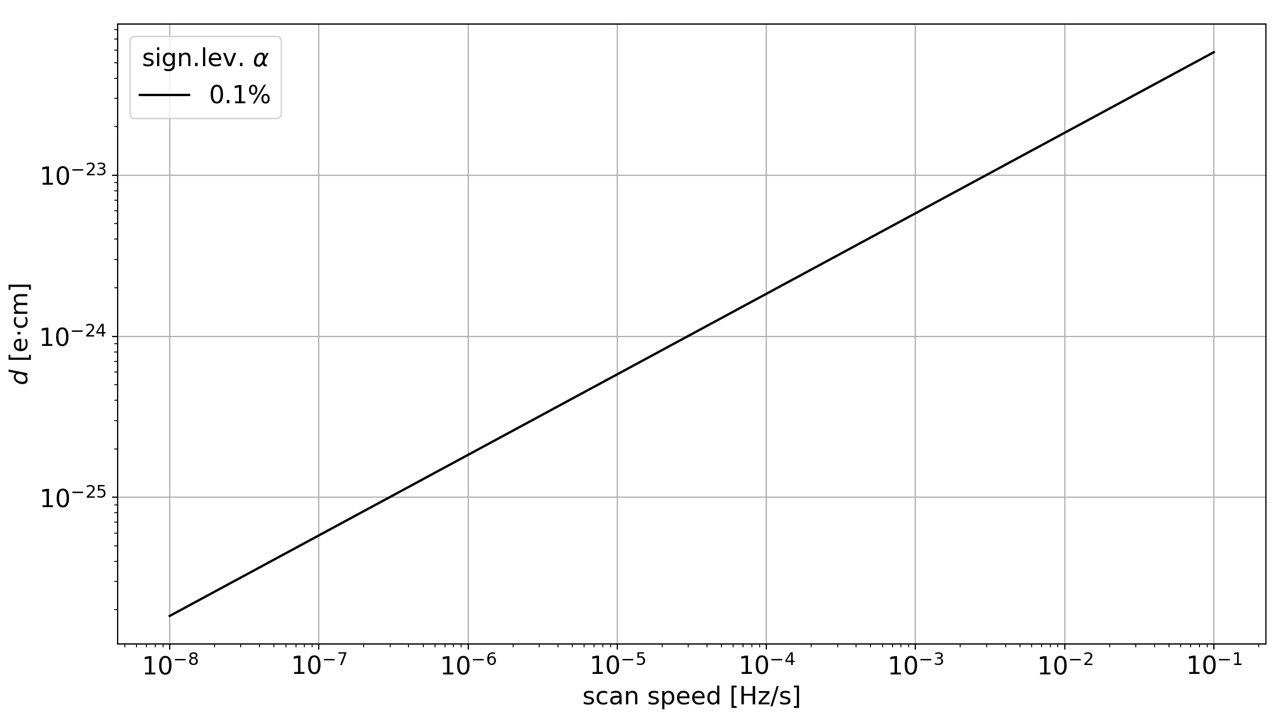
\includegraphics[width=\linewidth]{YVSsignal_vs_scan_speed}
	\caption{EDM estimate projection for the pilot experiment.
		\label{fig:Aksentev:Estimates2026:Fig4}
	}
\end{figure}


\begin{acknowledgments}
This work was supported by the Russian Science Foundation, grant
No.~25-72-30005 (\url{https://rscf.ru/project/25-72-30005/}).
\end{acknowledgments}

\bibliography{references}

\end{document}
